\chapter{Preparation for H(Inv) decays in the VBF channel with CMS parked data}
\label{CHAPTER:PreparationParkedDataAnalysis}

%Status: DONE (reviewed J.Pela x1)

The Run I \gls{CMS} \gls{VBF} Higgs to invisible analysis was performed over two overlapping datasets. The promptly reconstructed data became available almost immediately after recording and its analysis was already presented in chapter \ref{CHAPTER:PromptDataAnalysis}, and became known as the Run I \textit{prompt analysis}. Simultaneously, a second data stream was recorded with lower trigger thresholds which only became available for analysis after the full \gls{LHC} Run I was finished. This chapter describes the studies made to prepare the Run I \textit{parked analysis} over this additional dataset. 

A description of the studies performed to develop the trigger conditions used to record data for the \gls{VBF} Higgs to invisible analysis can be found in section \ref{SECTION:PreparationParkedDataAnalysis_ParkedTriggerDevelopment}. This study was extend to create a condition to select \gls{VBF} Higgs events independently of the final state.

The lower trigger thresholds required a re-optimization of the analysis event selection. Due to the lack of enough simulated event statistics the \textit{prompt analysis} was tuned to suppress the selection of \gls{QCD} multi-jet processes to a negligible level. The ability to lower the selection thresholds to take advantage of the lower parked data trigger requirements was therefore  limited by our understanding of the \gls{QCD} multi-jet background. Having a \gls{MC} description of these type of events would allow easier threshold optimization and create the opportunity for the analysis to evolve to a shape based or \gls{MVA} based analysis.

The production and characterization of \gls{QCD} multi-jet samples with \gls{VBF} characteristics and real \gls{MET} is described in section \ref{SECTION:PreparationParkedDataAnalysis_QCDVBFMET}. Further studies of possible approaches to suppress the \gls{QCD} multi-jet background are presented in sections \ref{SECTION:PreparationParkedDataAnalysis_DijetMETSystemVars} and \ref{SECTION:PreparationParkedDataAnalysis_TrackDistributionVariables}.

%%%%%%%%%%%%%%%%%%%%%%%%%%%%%%%%%%%%%%%%%%%%%%%%%%%%%%%%%%%%%%%%%%%%%%%%%%%%%%%%%%%%
%%% SECTION
%%%%%%%%%%%%%%%%%%%%%%%%%%%%%%%%%%%%%%%%%%%%%%%%%%%%%%%%%%%%%%%%%%%%%%%%%%%%%%%%%%%%
\section{L1T parked trigger development}
\label{SECTION:PreparationParkedDataAnalysis_ParkedTriggerDevelopment}

%Status: DONE (reviewed J.Pela x1)

The first step of any analysis is defining or selecting a trigger to collect data. This trigger should have a high signal efficiency while recording an acceptable rate.

At the beginning of 2012 the possibility of recording data without promptly reconstructing it was introduced. This additional data is now known as \textit{parked data}. The \gls{CMS} \gls{VBF} Higgs to invisible analysis saw this as an opportunity to develop a secondary set of triggers with lower thresholds to allow more signal to be collected when compared with the already developed prompt trigger. As this effort developed it became clear that an inclusive trigger that would record \gls{VBF} events regardless of final state could be implemented.

%%%%%%%%%%%%%%%%%%%%%%%%%%%%%%%%%%%%%%%%%%%%%%%%%%%%%%%%%%%%%%%%%%%%%%%%%%%%%%%%%%%%
%%% SUBSECTION
%%%%%%%%%%%%%%%%%%%%%%%%%%%%%%%%%%%%%%%%%%%%%%%%%%%%%%%%%%%%%%%%%%%%%%%%%%%%%%%%%%%%
\subsection{VBF Higgs to Invisible Higgs Level 1 trigger development}
\label{SUBSECTION:ParkedDataAnalysis_ParkedTriggerDevelopment_VBFHiggsInvisibleTrigger}

%Status: DONE (reviewed J.Pela x1)

Data recorded during the special high \gls{PU} run in late 2011, was used to study \gls{L1T} trigger algorithms to be used during the 2012 proton run. During this \gls{LHC} fill the average \gls{PU} was of $\approx 30$ simultaneous interactions. 

The investigated algorithms select the typical topology of our signal. They look for events with \gls{MET} and and two jets located in opposite sides of the detector by requiring $\eta_{jet1}\times\eta_{jet2}<0$, large pseudo-rapidity separation of at least $\Delta\eta_{jj}>3$. The possibility of using $\Delta\phi_{jj}$ was also studied but was disfavoured since it could lead to lower signal efficiency in some \gls{BSM} models.

The conditions expected for early 2012 were of instantaneous luminosity of $5 \times 10^{33}\,\centi\meter^{-2}\second^{-1}$ and an average \gls{PU} of 28 interactions (scenario A). For late 2012 conditions were expected to increase to instantaneous luminosity of $7 \times 10^{33}\,\centi\meter^{-2}\second^{-1}$ and an average \gls{PU} of 32 interactions (scenario B).

Algorithm parameters were optimized for both this scenarios of \gls{LHC} running and considering several benchmark \gls{L1T} rates. The proposed target rate for the algorithm was assumed to be $2\,\kilo\Hz$, the additional working points were calculated with the intention to adjust the selection cuts according to higher or lower bandwidth available on the menu. The two key variables are $\pt^{\text{jets}}$ and the \gls{MET} and were optimized separately. Each of these variables was set in turn to the lowest reasonable value while the other was scanned until the necessary rate value was achieved.  Results for scenario A can be found in table \ref{TABLE:ParkedDataAnalysis_L1TParkedTriggerDevelopment_Rate5E33} and for scenario B in table \ref{TABLE:ParkedDataAnalysis_L1TParkedTriggerDevelopment_Rate7E33}.

\begin{table}[!htb]
\begin{minipage}{.5\linewidth}
  \centering
  \begin{tabular}{|c||c|c|c|c|}
  \hline
  \multicolumn{5}{|c|}{MET [GeV] ($\pt^{\text{jets}} > 20\,\GeV$)} \\
  \hline\hline
  $\Delta\phi$ & no cut & 2.5 & 2.1 & 1.8 \\
  \hline
   $10\,\kHz$  &     32 &  32 &  32 &  32 \\
    $5\,\kHz$  &     35 &  35 &  35 &  35 \\
  \hline\hline
    $2\,\kHz$  &     41 &  41 &  41 &  41 \\
  \hline\hline
    $1\,\kHz$  &     47 &  47 &  47 &  46 \\
  $0.5\,\kHz$  &     54 &  54 &  54 &  53 \\
  \hline
  \end{tabular}
\end{minipage}%
\begin{minipage}{.5\linewidth}
  \centering
  \begin{tabular}{|c||c|c|c|c|}
  \hline
  \multicolumn{5}{|c|}{$\pt^{\text{jets}}$ [GeV] ($\text{MET}>30\,\GeV$)} \\
  \hline
  $\Delta\phi$ & no cut & 2.5 & 2.1 & 1.8 \\
  \hline\hline
   $10\,\kHz$  &     28 &  28 &  24 &  24 \\
    $5\,\kHz$  &     32 &  32 &  32 &  32 \\
  \hline\hline
    $2\,\kHz$  &     52 &  48 &  44 &  44 \\
  \hline\hline
    $1\,\kHz$  &     68 &  68 &  64 &  64 \\
  $0.5\,\kHz$  &     92 &  92 &  88 &  88 \\
  \hline
  \end{tabular}
\end{minipage} 
\caption{Tables showing the \gls{L1T} rate for different selection criteria for $5 \times 10^{33}\,\centi\meter^{-2}\second^{-1}$ and an average \gls{PU} of 28 interactions (scenario A). In selected events the leading two jets is in opposite sides of the detector. On the left table the \gls{MET} cut is calculated while requiring the two leading jets to have $\pt^{\text{jets}} > 20\,\GeV$. Similarly, on the right table $\pt^{\text{jets}}$ cut is calculated while requiring $\text{MET}>30\,\GeV$.}
\label{TABLE:ParkedDataAnalysis_L1TParkedTriggerDevelopment_Rate5E33}
\end{table}

\begin{table}[!htb]
\begin{minipage}{.5\linewidth}
  \centering
  \begin{tabular}{|c||c|c|c|c|}
  \hline
  \multicolumn{5}{|c|}{MET [GeV] ($\pt^{\text{jets}}>20\,\GeV$)} \\
  \hline\hline
  $\Delta\phi$ & no cut & 2.5 & 2.1 & 1.8 \\
  \hline
   $10\,\kHz$  &     36 &  36 &  36 &  36 \\
    $5\,\kHz$  &     40 &  40 &  40 &  40 \\
  \hline\hline
    $2\,\kHz$  &     47 &  47 &  47 &  46 \\
  \hline\hline
    $1\,\kHz$  &     54 &  54 &  54 &  54 \\
  $0.5\,\kHz$  &     67 &  66 &  66 &  64 \\
  \hline
  \end{tabular}
\end{minipage}%
  \begin{minipage}{.5\linewidth}
    \centering
  \begin{tabular}{|c||c|c|c|c|}
  \hline
  \multicolumn{5}{|c|}{$\pt^{\text{jets}}$ [GeV] ($\text{MET}>30\,\GeV$)} \\
  \hline
  $\Delta\phi$ & no cut & 2.5 & 2.1 & 1.8 \\
  \hline\hline
   $10\,\kHz$  &     32 &  32 &  32 &  32 \\
    $5\,\kHz$  &     40 &  40 &  40 &  40 \\
  \hline\hline
    $2\,\kHz$  &     64 &  60 &  60 &  56 \\
  \hline\hline
    $1\,\kHz$  &     76 &  76 &  76 &  76 \\
  $0.5\,\kHz$  &    100 & 100 &  96 &  92 \\
  \hline
  \end{tabular}
\end{minipage} 
\caption{Tables showing the \gls{L1T} rate for different selection criteria for $7 \times 10^{33}\,\centi\meter^{-2}\second^{-1}$ and an average \gls{PU} of 32 interactions (scenario B). In selected events the leading two jets is in opposite sides of the detector. On the left table the \gls{MET} cut is calculated while requiring the two leading jets to have $\pt^{\text{jets}} > 20\,\GeV$. Similarly, on the right table $\pt^{\text{jets}}$ cut is calculated while requiring $\text{MET}>30\,\GeV$.}
\label{TABLE:ParkedDataAnalysis_L1TParkedTriggerDevelopment_Rate7E33}
\end{table}

These results were used to define working points for this trigger, which were proposed to the \glsreset{TSG}
to be included on \gls{L1T} Menus. Proposed trigger options were:
\begin{itemize}
\item Algorithm A: Lead dijet (opp. sides + $\pt^{\text{jets}}>20\,\GeV$ + $\Delta\eta_{jj}>3$) + $\text{MET}>40\,\GeV$
\item Algorithm B: Lead dijet (opp. sides + $\pt^{\text{jets}}>50\,\GeV$ + $\Delta\eta_{jj}>3$) + $\text{MET}>30\,\GeV$
\end{itemize}

It can be observed that with the predicted increase of instantaneous luminosity and \gls{PU} from scenario A to scenario B, the necessary rate for such proposed algorithms could escalate up to $\approx 5\,\kilo\Hz$. For the rate to be maintained at $2\,\kilo\Hz$ the value of the MET cut in algorithm A would have to be raised to $47\,\GeV$ and the value of $\pt^{\text{jets}}$ cut in algorithm B would have to increase to $64\,\GeV$.

%%%%%%%%%%%%%%%%%%%%%%%%%%%%%%%%%%%%%%%%%%%%%%%%%%%%%%%%%%%%%%%%%%%%%%%%%%%%%%%%%%%%
%%% SUBSECTION
%%%%%%%%%%%%%%%%%%%%%%%%%%%%%%%%%%%%%%%%%%%%%%%%%%%%%%%%%%%%%%%%%%%%%%%%%%%%%%%%%%%%
\subsection{VBF Higgs inclusive Level 1 trigger development}
\label{SUBSECTION:ParkedDataAnalysis_ParkedTriggerDevelopment_InclusiveHiggsTrigger}

%Status: DONE

It would be desirable to have a dedicated \gls{VBF} Higgs inclusive \gls{L1T} trigger that would be decay independent. Such an algorithm would allow analysts to have a single trigger for all \gls{VBF} produced Higgs decay signatures, which would imply less systematics in their comparison. Additionally, if an algorithm is used by more analyses it will become better understood.

When selecting events based only on the presence of a dijet with \gls{VBF} characteristics we can remove the dependency on the Higgs decay. This approach would be suitable since it ignores the Higgs decays themselves. Since we are not making any assumptions of the Higgs model, we could study all possible decays even those predicted by yet to be defined models with a single trigger. Thus, it would be a model-independent trigger.

This trigger can also be used for analysis of WW scattering, which in the case of the absence of the now discovered Higgs boson would allow to eventually exclude the standard model itself. Since without a Higgs boson this process probability would become larger than unity at the $\TeV$ scale.
%TODO: need reference here.

Such a trigger would have to select two forward jets with \gls{VBF} characteristics, and would be limited to what is possible to implement on the current \gls{L1T} hardware. The following variables were considered to suppress the algorithm rate by constrain the dijet system: dijet invariant mass, dijet transverse invariant mass ($M_{T}$), and event \gls{HT}. For this study we always require a \gls{L1T} dijet with both jets in opposite sides of the detector with $\Delta\eta>3$. The selected jets \pt is scanned and \gls{L1T} algorithm rate is calculated for a grid of points of each considered variable.

%%%%%%%%%%%%%%%%%%%%%%%%%%%%%%%%%%%%%%%%%%%%%%%%%%%%%%%%%%%%%%%%%%%%%%%%%%%%%%%%%%%%
%%% SUBSUBSECTION
%%%%%%%%%%%%%%%%%%%%%%%%%%%%%%%%%%%%%%%%%%%%%%%%%%%%%%%%%%%%%%%%%%%%%%%%%%%%%%%%%%%%
\subsubsection{Dijet invariant mass}

%Status: DONE

The for \gls{VBF} processes the outgoing dijet is expected to have high invariant mass making this quantity a possible handle at in a \gls{L1T} trigger algorithm. Calculation of dijet invariant mass was not implemented in the \gls{L1T} hardware but according to trigger experts it was in principle possible. Unfortunately, to obtain acceptable rates the required threshold for jet $p_T$ and $M_{jj}$ would reject almost all \gls{SM} \gls{VBF} Higgs signal.

%%%%%%%%%%%%%%%%%%%%%%%%%%%%%%%%%%%%%%%%%%%%%%%%%%%%%%%%%%%%%%%%%%%%%%%%%%%%%%%%%%%%
%%% SUBSUBSECTION
%%%%%%%%%%%%%%%%%%%%%%%%%%%%%%%%%%%%%%%%%%%%%%%%%%%%%%%%%%%%%%%%%%%%%%%%%%%%%%%%%%%%
\subsubsection{Dijet transverse invariant mass}

%Status: DONE

The dijet transverse mass was also considered and was proved to be more effective at suppressing \gls{QCD} multi-jet events. Again, this quantity is not implemented on the \gls{L1T} hardware but could be implemented. A possible working point for scenario A was obtained with a predicted \gls{L1T} rate of $5\kilo\hertz$. Events would be selected with at least one dijet with $\Delta\eta>3$ and $M_T>50\,\GeV$ where both jets have $p_T \sim 45\,\GeV$ and are in opposite sides of the detector. The expected signal efficiency was calculated to be $\approx 70\%$ for a \gls{SM} \gls{VBF} Higgs with $m_H=125\,\GeV$ decaying to $\tau\tau$.

%%%%%%%%%%%%%%%%%%%%%%%%%%%%%%%%%%%%%%%%%%%%%%%%%%%%%%%%%%%%%%%%%%%%%%%%%%%%%%%%%%%%
%%% SUBSUBSECTION
%%%%%%%%%%%%%%%%%%%%%%%%%%%%%%%%%%%%%%%%%%%%%%%%%%%%%%%%%%%%%%%%%%%%%%%%%%%%%%%%%%%%
\subsubsection{Event scaler sum of the transverse hadronic energy}

%Status: DONE

The event scaler sum of the transverse hadronic energy is the sum of the energy of all \gls{L1T} jets in the event. This variable has the advantage of being already implemented in the \gls{L1T} hardware. Again, a possible working point for scenario A was obtained with a predicted \gls{L1T} rate of $5\kilo\hertz$. Events would be selected with $HT>100\,\GeV$ and with at least one dijet with $\Delta\eta>3$ where both jets have $p_T \sim 40\,\GeV$ and are in opposite sides of the detector. The expected signal efficiency was calculated to be $\approx 98\%$ for a \gls{SM} \gls{VBF} Higgs with $m_H=125\,\GeV$ decaying to $\tau\tau$. A plot of the scan over \gls{L1T} $\pt^{jets}$ for $HT>100\,\GeV$ can be found in figure \ref{FIGURE:ParkedDataAnalysis_ParkedTriggerDevelopment_PU28_5e33_RateFBDijetDEtaDPhi00HT100}.

\begin{figure}[ht]
\centering
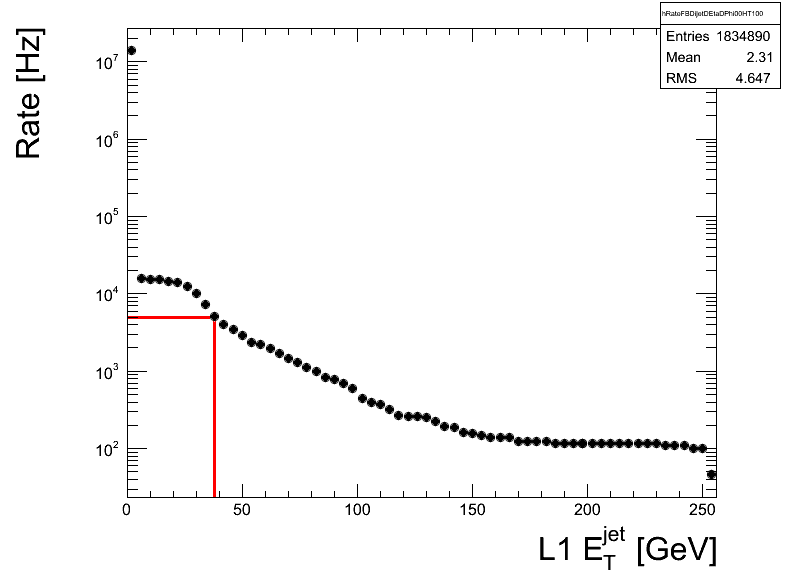
\includegraphics[width=0.60\textwidth]{Chapter07/ParkedDataTriggerDevelopment/Images/PU28_5e33_RateFBDijetDEtaDPhi00HT100.png}
\caption{Level 1 rate as a function of dijet $p_T^{jets}$ while selecting events with at least one dijet with $\Delta\eta>3$ where are in opposite sides of the detector and $HT>100\,\GeV$ for scenario A. Results based on data from the high pileup special run taken late 2011. The red lines indicate the selected working point of \gls{L1T} rate of $5\,\kilo\hertz$ resulting in a $p_T^{jets} \gtrsim 40\,\GeV$ threshold.}
\label{FIGURE:ParkedDataAnalysis_ParkedTriggerDevelopment_PU28_5e33_RateFBDijetDEtaDPhi00HT100}
\end{figure}

%%%%%%%%%%%%%%%%%%%%%%%%%%%%%%%%%%%%%%%%%%%%%%%%%%%%%%%%%%%%%%%%%%%%%%%%%%%%%%%%%%%%
%%% SUBSECTION
%%%%%%%%%%%%%%%%%%%%%%%%%%%%%%%%%%%%%%%%%%%%%%%%%%%%%%%%%%%%%%%%%%%%%%%%%%%%%%%%%%%%
\subsection{Final proposal}

%Status: DONE

The \gls{L1T} algorithm selecting \gls{MET} bigger than $40\,\GeV$ was unprescaled in the trigger menus used during Run I, it was decided to use this algorithm as seed for the invisible component of \gls{VBF} Higgs decays. Thus avoiding the additional complication of having to implement a dijet plus \gls{MET} \gls{L1T} algorithm for minimal threshold gain. For the \gls{VBF} channels with visible decays and considering the findings of this study, a similar simplified approach was taken. Depending on the delivered instantaneous luminosity and prescale events with \gls{HT} bigger than 150 or $170\,\GeV$ would be selected. The developed inclusive \gls{VBF} Higgs \gls{HLT} path was seeded by a logical or the these three \gls{L1T} seeds.

%%%%%%%%%%%%%%%%%%%%%%%%%%%%%%%%%%%%%%%%%%%%%%%%%%%%%%%%%%%%%%%%%%%%%%%%%%%%%%%%%%%%
%%% SECTION
%%%%%%%%%%%%%%%%%%%%%%%%%%%%%%%%%%%%%%%%%%%%%%%%%%%%%%%%%%%%%%%%%%%%%%%%%%%%%%%%%%%%
\section{Monte Carlo simulation of QCD multi-jet events with VBF jets and MET}
\label{SECTION:PreparationParkedDataAnalysis_QCDVBFMET}

% %%%%%%%%%%%%%%%%%%%%%%%%%%%%%%%%%%%%%%%%%%%%%%%%%%%%%%%%%%
% QCD VFB + MET samples
% %%%%%%%%%%%%%%%%%%%%%%%%%%%%%%%%%%%%%%%%%%%%%%%%%%%%%%%%%%
% 20140204_ICVBFHiggs_JPela_VBFQCD.pdf (plot on the AN)
% 20140506_ICVBFHiggs_JPela.pdf (selection test)
% 
% Something odd here
% /home/hep/jca10/work/vbfinv/ws08/CMSSW_5_3_11/src/UserCode/ICHiggsTauTau/Analysis/HiggsNuNu

%Status: DONE

Simulating and reconstructing quantities of \gls{QCD} multi-jet events comparable to the ones produced at the \gls{LHC} experiments is impractical. At every second of \gls{LHC} physics operation several millions of bunch crossings happen, each one able to create several simultaneous collisions. With the currently available hardware it takes in excess of one minute to fully simulate one of such bunch crossings. Further more, most of this events have only low transverse momentum collisions and are unlikely to be picked up by any physics analysis selections.

This constraints lead to \gls{QCD} multi-jets events being simulated in $p_T$ hats, where the first simulated collision outgoing particles summed $p_T$ is generated within a predefined range. Then several other collisions are added to the event as \gls{PU}. This additional collisions are generated without any constraints in $p_T$. 

This binned method allows the user to have access to \gls{QCD} hard scattering samples with increasing energies. Such event samples allow studying the contribution of each \gls{QCD} multi-jet energy range to an hypothetical analysis selection. As a practical example we do not need to look over millions of \gls{QCD} events to find high energy jets. We can just start from the highest \gls{QCD} $p_T$ hat and add lower bins until the contributing to the event selection is negligible. On the other hand, analysis like the \gls{CMS} \gls{VBF} Higgs to invisible analysis, searches for event topologies with low energy jets and/or \gls{MET}. In this cases, available inclusive \gls{QCD} samples will not have enough statistics to provide insight into this backgrounds behaviour.

The signal for this analysis has well separated jets in $\eta$ and large \gls{MET}. Generating \gls{QCD} multi-jet events with such characteristics could allow us to simulate enough statistics to compare with the recorded data and would hopefully describe this background. To create such simulated event sample a generator level filter had to be implemented. Simulation was done using the \textsc{PYTHIA 6} \gls{MC} event generator where events would only be kept if at least one generator anti-$k_T$ dijet would be found with $p_T^{jets}>20\,\GeV$, $|\eta_{jets}|<5.0$, $\Delta\eta>3.2$ and $M_{jj}>700\,\GeV$. Additionally, the vectorial sum of all the neutrinos in the event was required to be bigger than $40\,\GeV$. 

Similarly to the official \gls{QCD} multi-jet samples, these new simulated data sets were produced in the same bins, covering the \pt range from 80 to $600\,\GeV$. Higher \pt bins where not simulated since the official samples already had enough equivalent luminosity to be directly compared to data. Table \ref{TABLE:PreparationParkedDataAnalysis_QCDVBFMET_KeyParameters} summarizes the key parameters for each produced $\pt$ hat.

\begin{table}[!htb]
\centering
\begin{tabular}{|c|r|c|r|c|c|}
\hline
\pt hat [$\GeV$] & \specialcell{Filter\\Efficiency} &  \specialcell{Produced\\Events} & \specialcell{Cross\\Section $[pb]$} & \specialcell{Equivalent Integrated\\Luminosity $[fb^{-1}]$} \\
\hline \hline
 80-120          &    0.000049 & 1614416 &  1033680 &  38.09 \\
120-170          &    0.000283 & 2051000 & 156293.3 &  44.79 \\
170-300          &    0.000987 & 1391500 & 34138.15 &  40.28 \\
300-470          &    0.002659 &  207840 & 1759.549 &  45.47 \\
470-600          &    0.004127 &  104675 & 113.8791 & 219.53 \\
\hline
\end{tabular}
\caption{Table of the key parameters of each simulated \gls{MC} event sample ordered by \pt hat.}
\label{TABLE:PreparationParkedDataAnalysis_QCDVBFMET_KeyParameters}
\end{table}

Each sub-sample has approximately twice the integrated luminosity recorded during Run I except the bin $470-600\,\GeV$ which had approximately ten times the equivalent luminosity. Figure \ref{FIGURE:PreparationParkedDataAnalysis_QCDVBFMET_RecovsGenMET} show the generator \gls{MET} versus the reconstructed \gls{PF} \gls{MET} for all the produced events after being reweighed by their respective cross section. 

\begin{figure}[!htb]
\centering
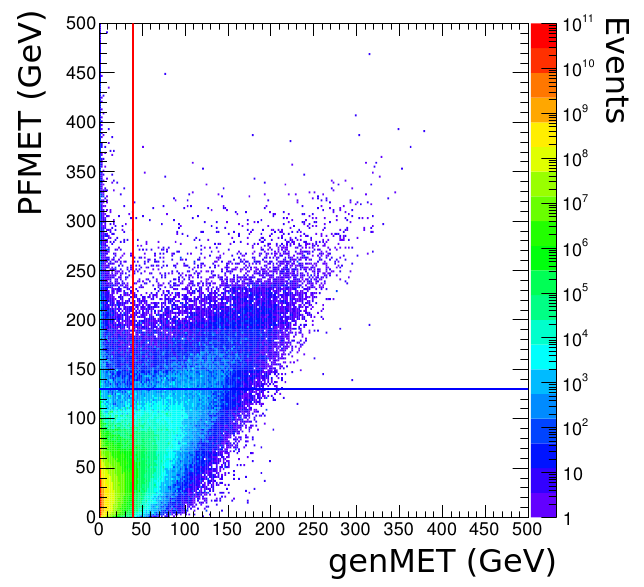
\includegraphics[width=0.55\textwidth]{Chapter05/ParkedDataPreparation/Images/Joao_140209_p11.png}
\caption{Reconstructed \gls{PF} \gls{MET} as a function of generator-level \gls{MET} in the inclusive \gls{QCD} multi-jet samples $80 < \hat{p_T} < 600$ GeV before any selection. The red is the generator cut applied to the privately produced \gls{QCD} multi-jet samples and the blue line is the \textit{prompt analysis} signal region \gls{PF} \gls{MET} requirement.}
\label{FIGURE:PreparationParkedDataAnalysis_QCDVBFMET_RecovsGenMET}
\end{figure}

Two event populations can be observed on this plot. The first along the diagonal of the two variables, when generator \gls{MET} is correctly reconstructed. The second population is along the vertical line at zero generator level \gls{MET}, which corresponds to events with miss reconstruction of \gls{MET}. When selecting events with \gls{PF} $\text{MET}>130\,\GeV$ the number of events with generator \gls{MET} bigger than $40\,\GeV$ is only 17-31\% of the total. Showing that most \gls{QCD} muli-jet events with high \gls{PF} \gls{MET} are miss measured. The produced \gls{QCD} multi-jet samples do not simulate miss measurement, but it was hoped at this time that a suitable event selection would suppress this type of events leaving only the real \gls{MET} topologies.

%%%%%%%%%%%%%%%%%%%%%%%%%%%%%%%%%%%%%%%%%%%%%%%%%%%%%%%%%%%%%%%%%%%%%%%%%%%%%%%%%%%%
%%% SUBSECTION
%%%%%%%%%%%%%%%%%%%%%%%%%%%%%%%%%%%%%%%%%%%%%%%%%%%%%%%%%%%%%%%%%%%%%%%%%%%%%%%%%%%%
\subsection{Pre-selection for data comparison}
\label{SECTION:PreparationParkedDataAnalysis_QCDVBFMETPreselection}

%Status: DONE

In an attempt to be use this samples effectively an event pre-selection was defined where the key variables of the \gls{VBF} Higgs to invisible analysis could be described by \gls{MC} simulation including the new \gls{QCD} multi-jet samples. If proven reliable it would be the ideal starting point for the optimization of a cut based analysis or to train a machine learning discriminator like a \gls{BDT}.

The approach taken was to methodically removed variable ranges on reference distributions where fake \gls{MET} events are likely to dominate. For data the trigger bit was required and for \gls{MC} simulated events the trigger reweighing was applied while he \textit{prompt analysis} lepton veto was applied to both. Events where only be accepted if the leading two jets have $p_T>50\,\GeV$, $|\eta|<4.7$ and their $\Delta\phi$ to the \gls{MET} vector is at least 1.5. Additionally, the dijet formed by these selected jets has $\Delta\eta>3.6$ and the significance of the \gls{MET} is at least 3. 

The \gls{QCD} multi-jet events passing this pre-selection were weighted so their total number would be the difference between data and all other estimate backgrounds estimated from \gls{MC} simulation. The selection signal efficiency for a \gls{SM} \gls{VBF} Higgs decay to invisible with $m_H=125\,\GeV$ was estimated to be 76\%. Figure \ref{FIGURE:PreparationParkedDataAnalysis_QCDVBFMET_PreSectionVariables} contains plots comparing data and \gls{MC} simulation for some of the key variables used in the \textit{prompt analysis} signal event selection.

%TODO: FIX THIS
\begin{figure}[!htb]
\vspace{-50px}
\centering
\subfloat[]{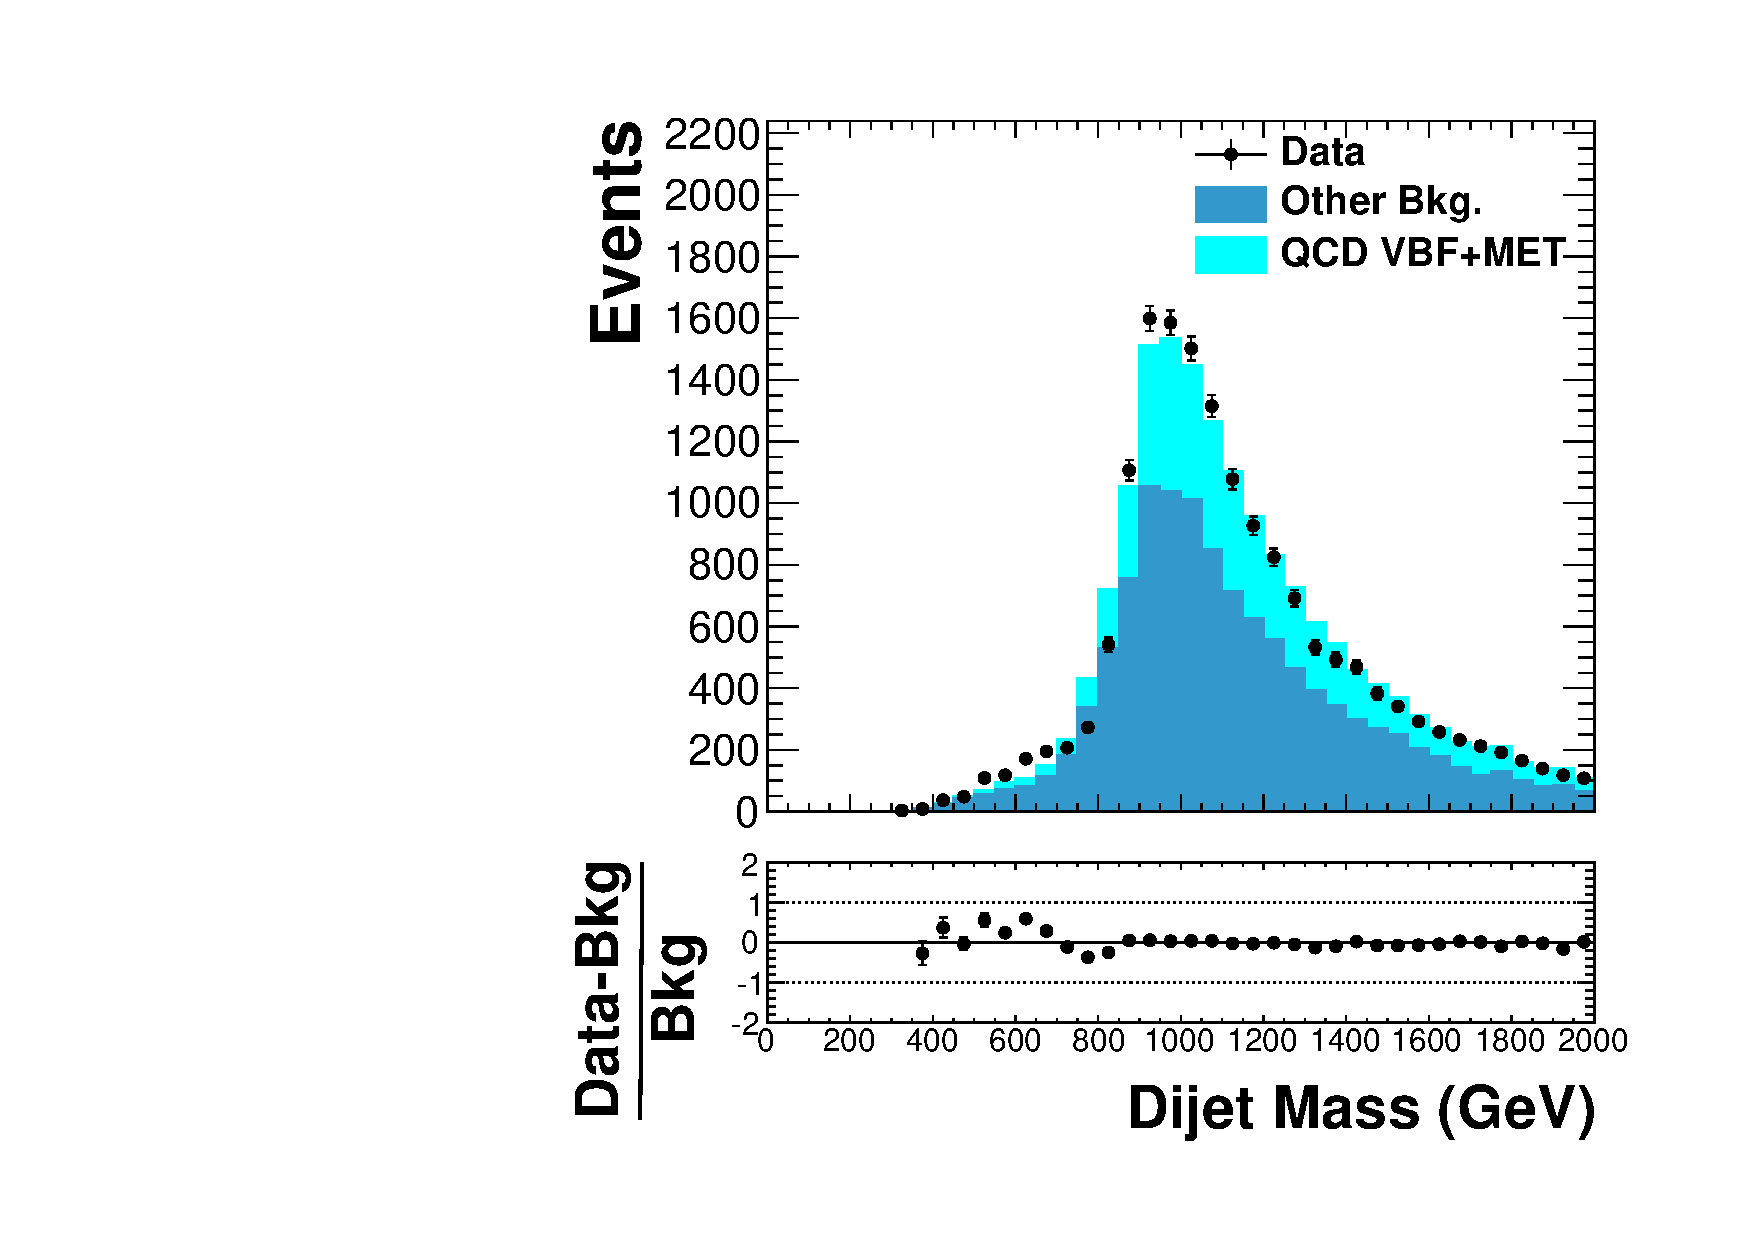
\includegraphics[width=0.45\linewidth]{Chapter06/QCD_VBFMET_Samples/PreSelection/Images//DEta3p6_MetSig3p0_MinDPhiJetsMet1p5/dijet_M.pdf}}
\subfloat[]{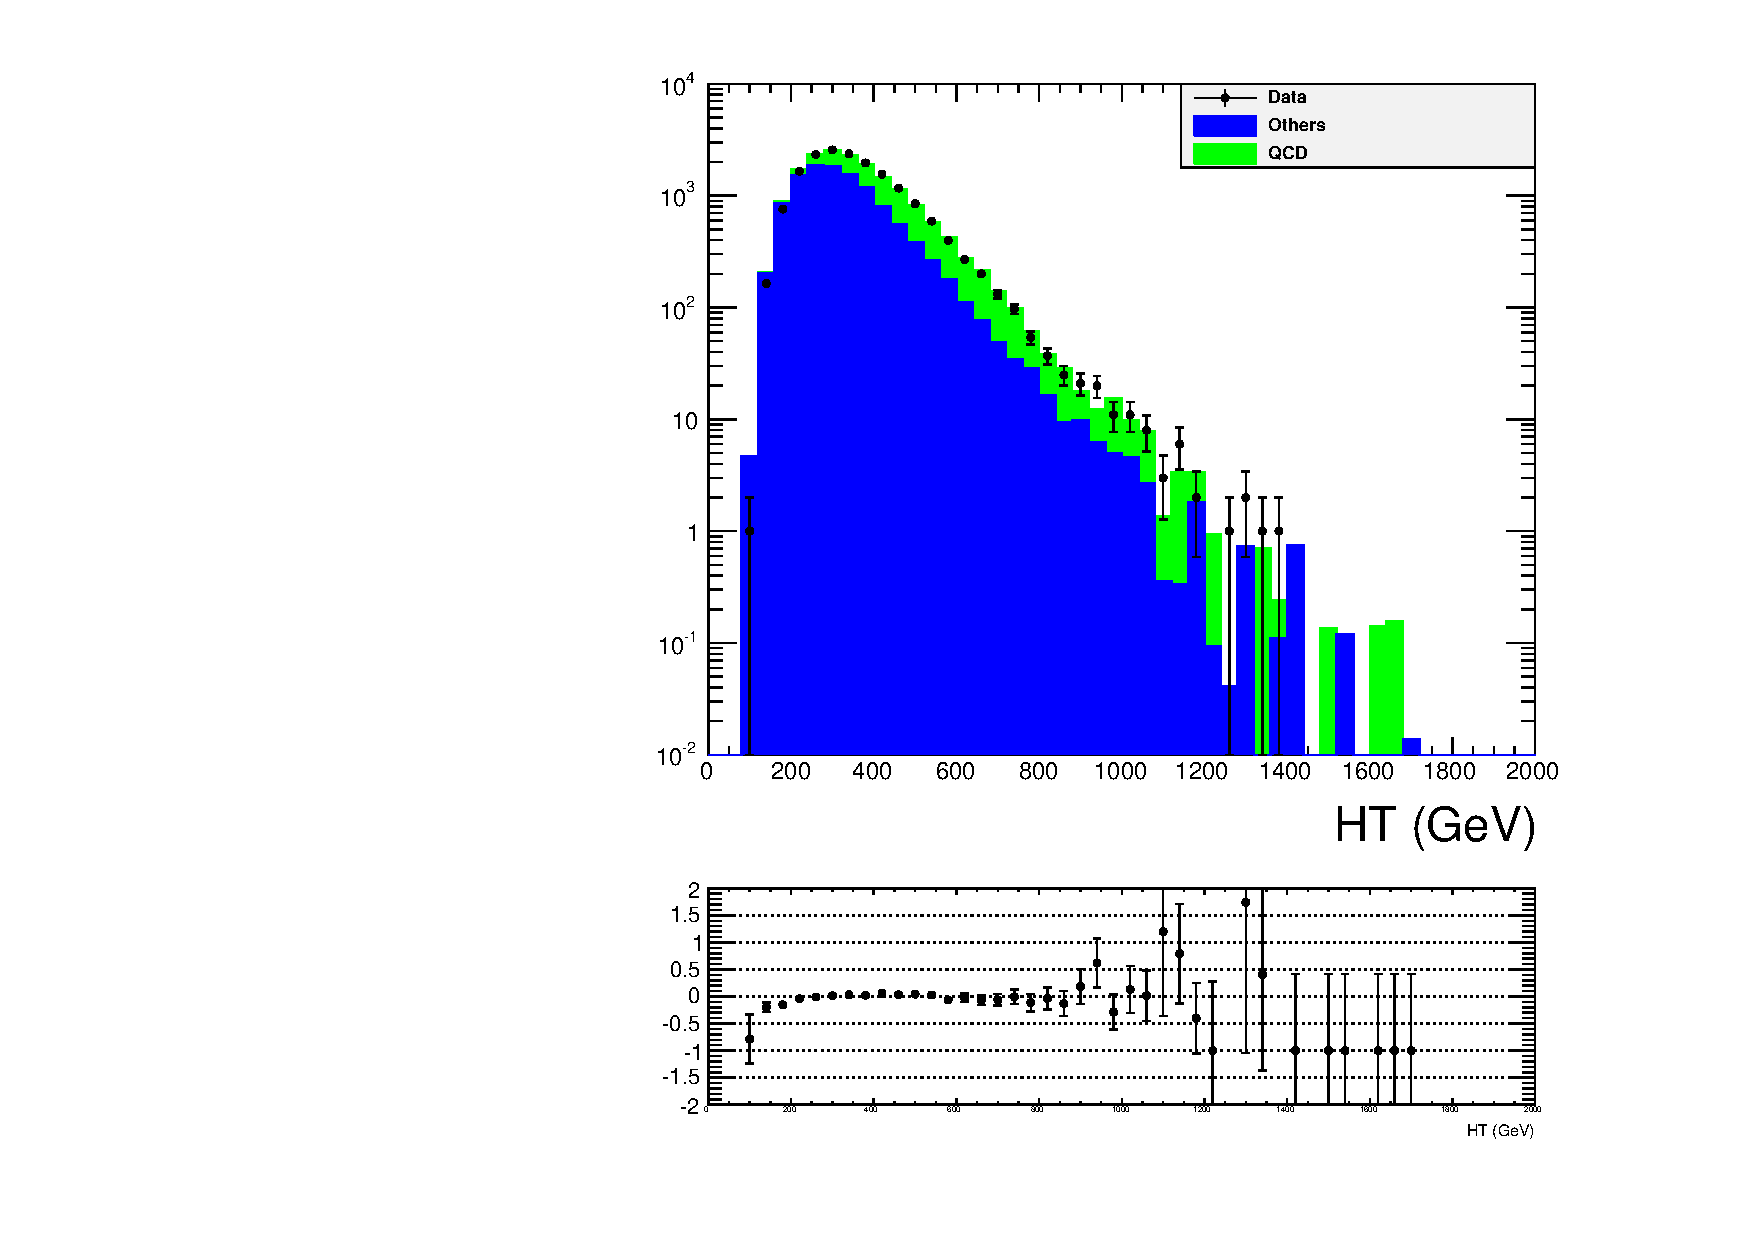
\includegraphics[width=0.45\linewidth]{Chapter06/QCD_VBFMET_Samples/PreSelection/Images//DEta3p6_MetSig3p0_MinDPhiJetsMet1p5/ht_LogY.pdf}} \\ 
\subfloat[]{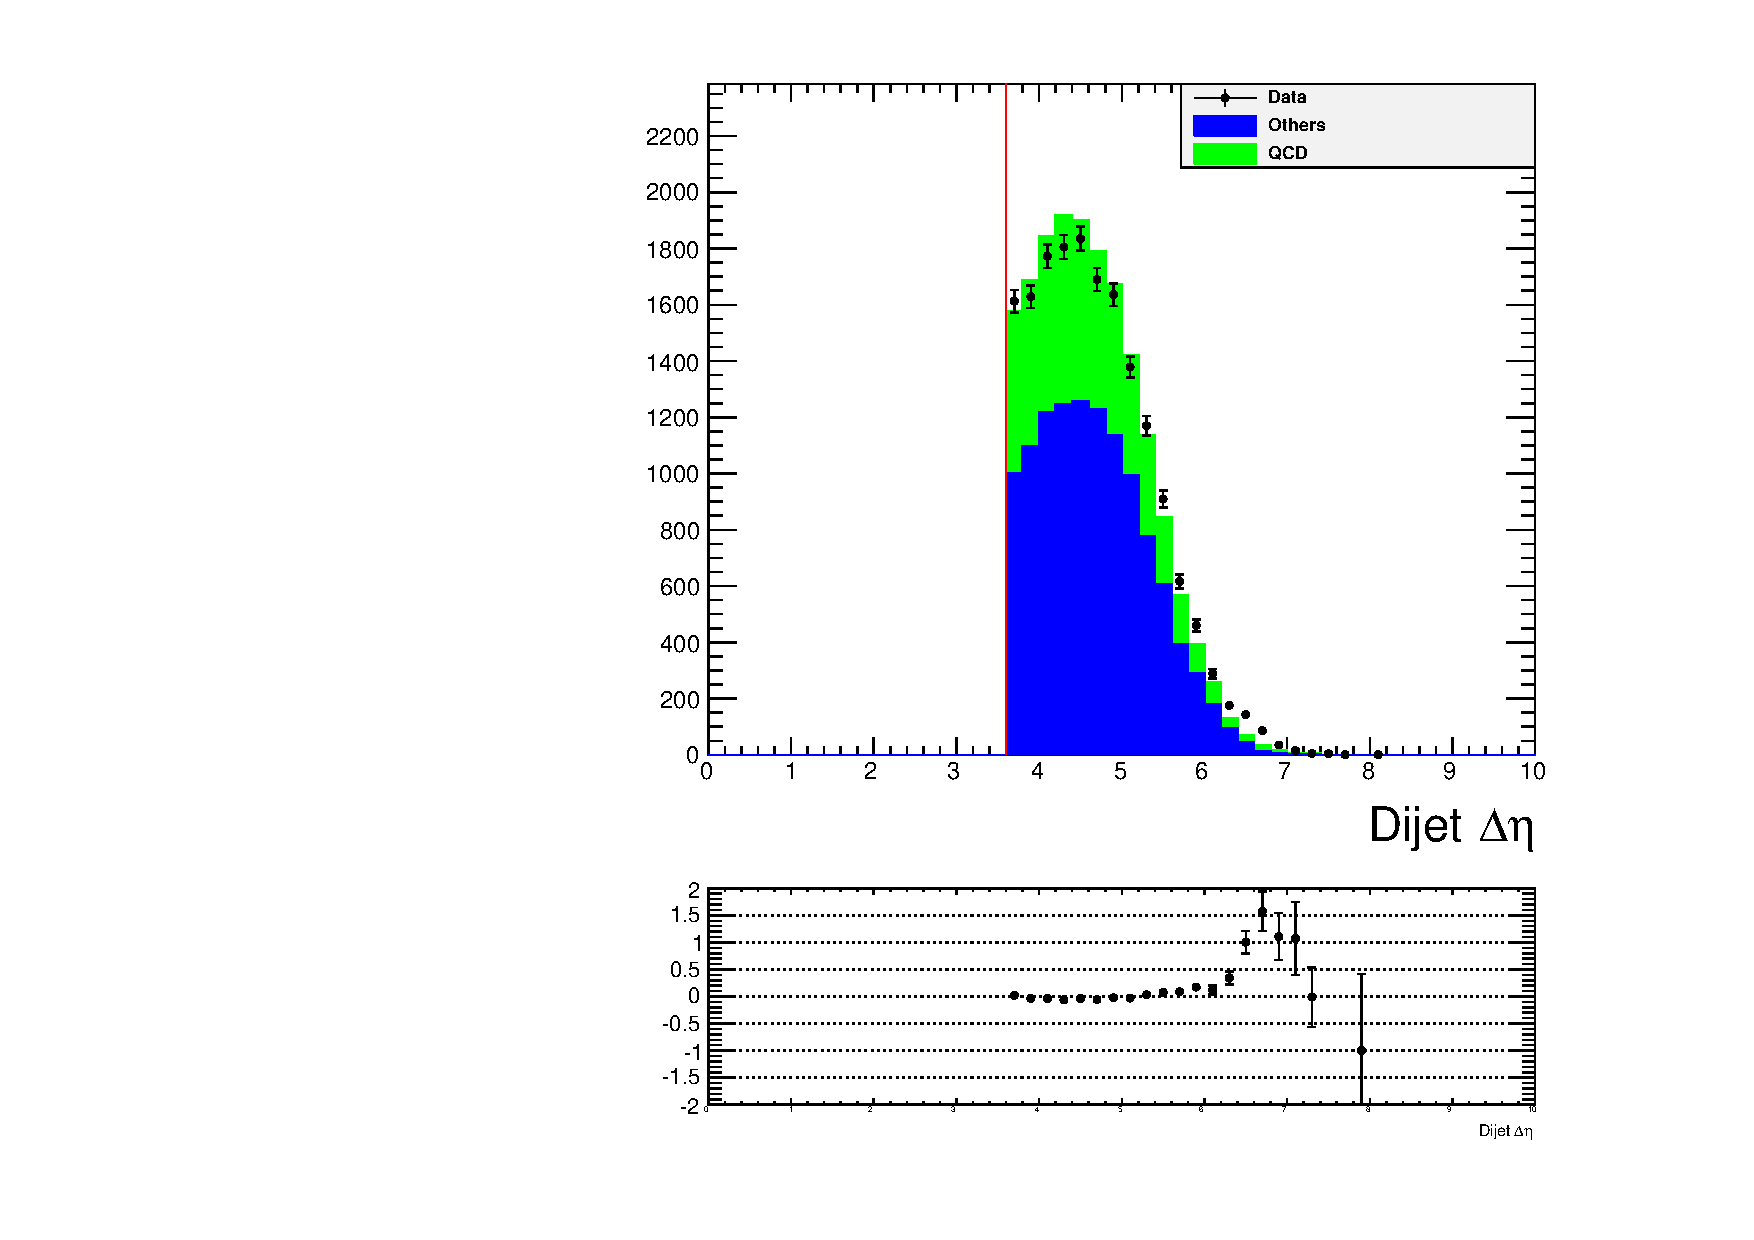
\includegraphics[width=0.45\linewidth]{Chapter06/QCD_VBFMET_Samples/PreSelection/Images//DEta3p6_MetSig3p0_MinDPhiJetsMet1p5/dijet_deta.pdf}}
\subfloat[]{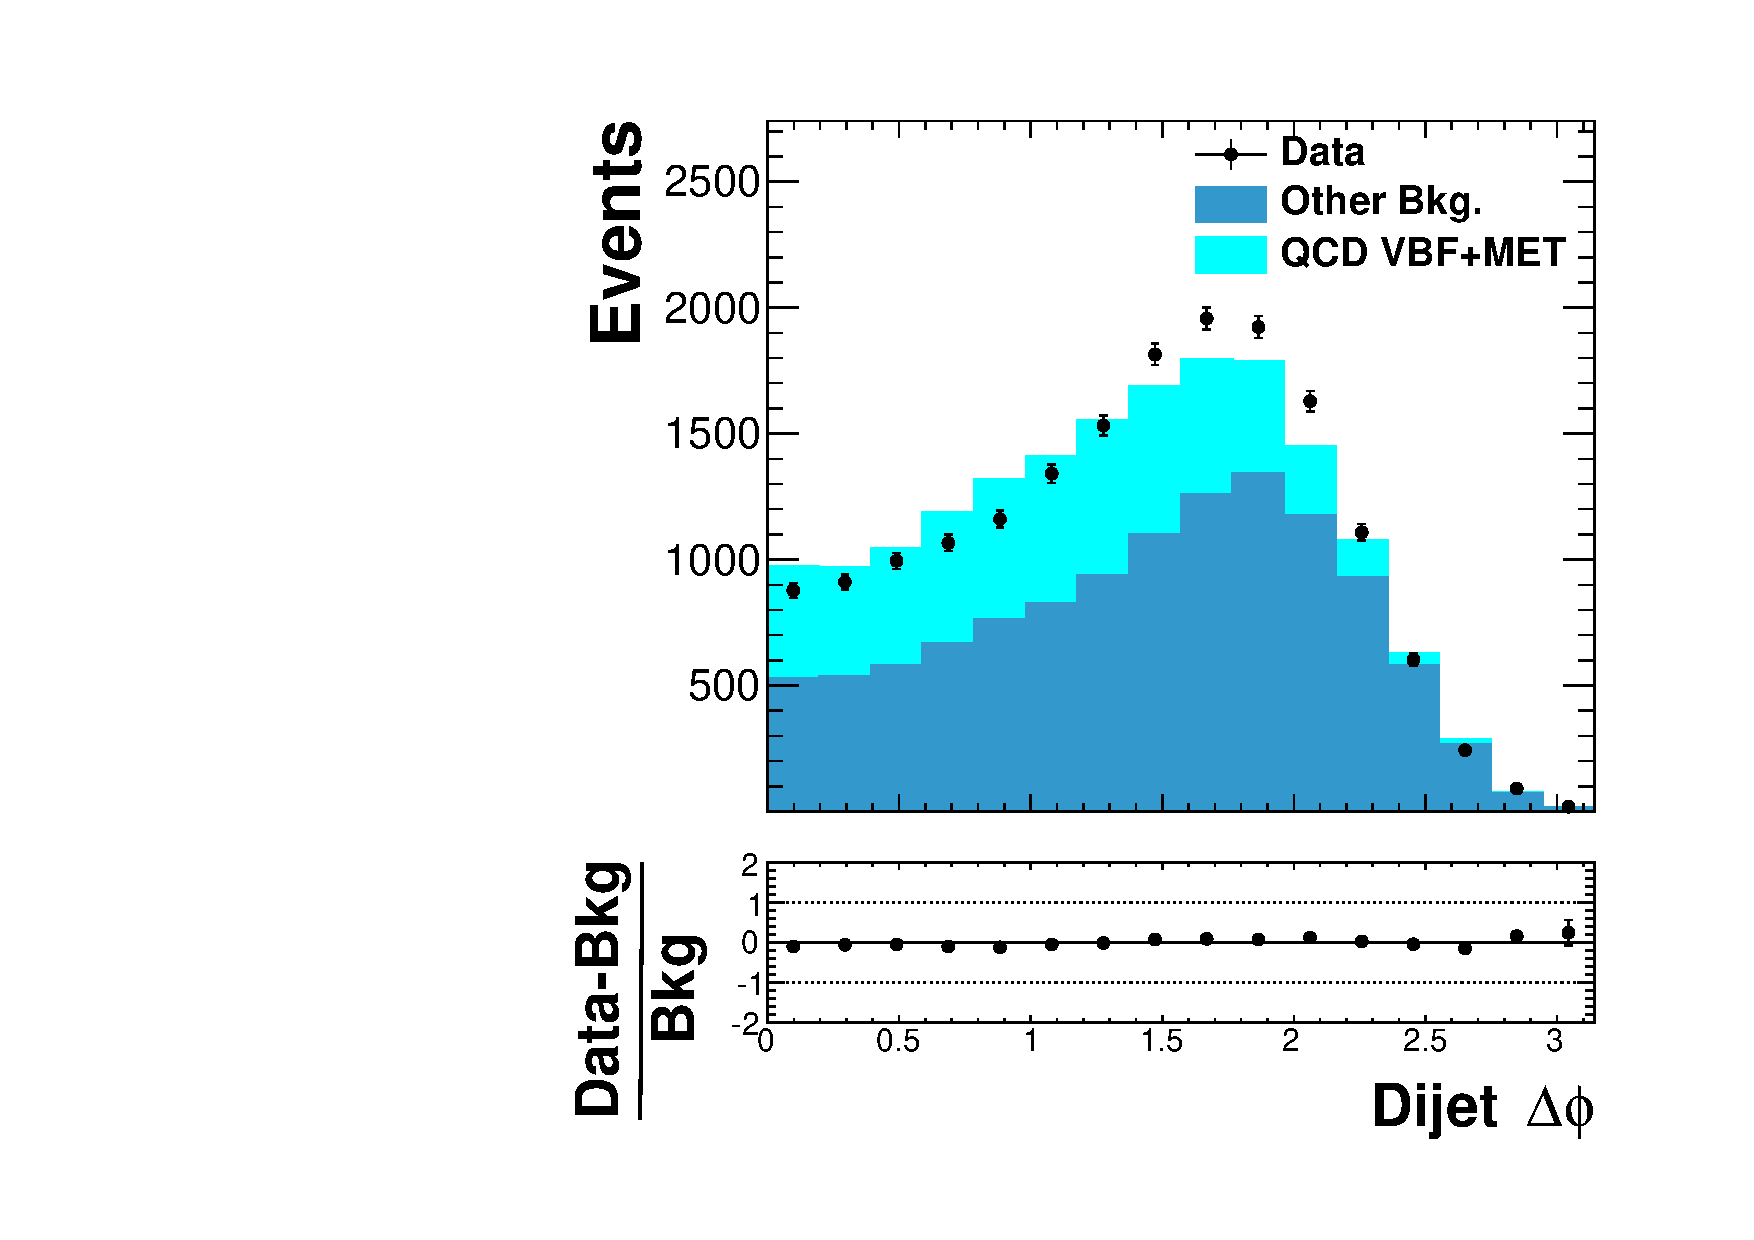
\includegraphics[width=0.45\linewidth]{Chapter06/QCD_VBFMET_Samples/PreSelection/Images//DEta3p6_MetSig3p0_MinDPhiJetsMet1p5/dijet_dphi.pdf}} \\ 
\subfloat[]{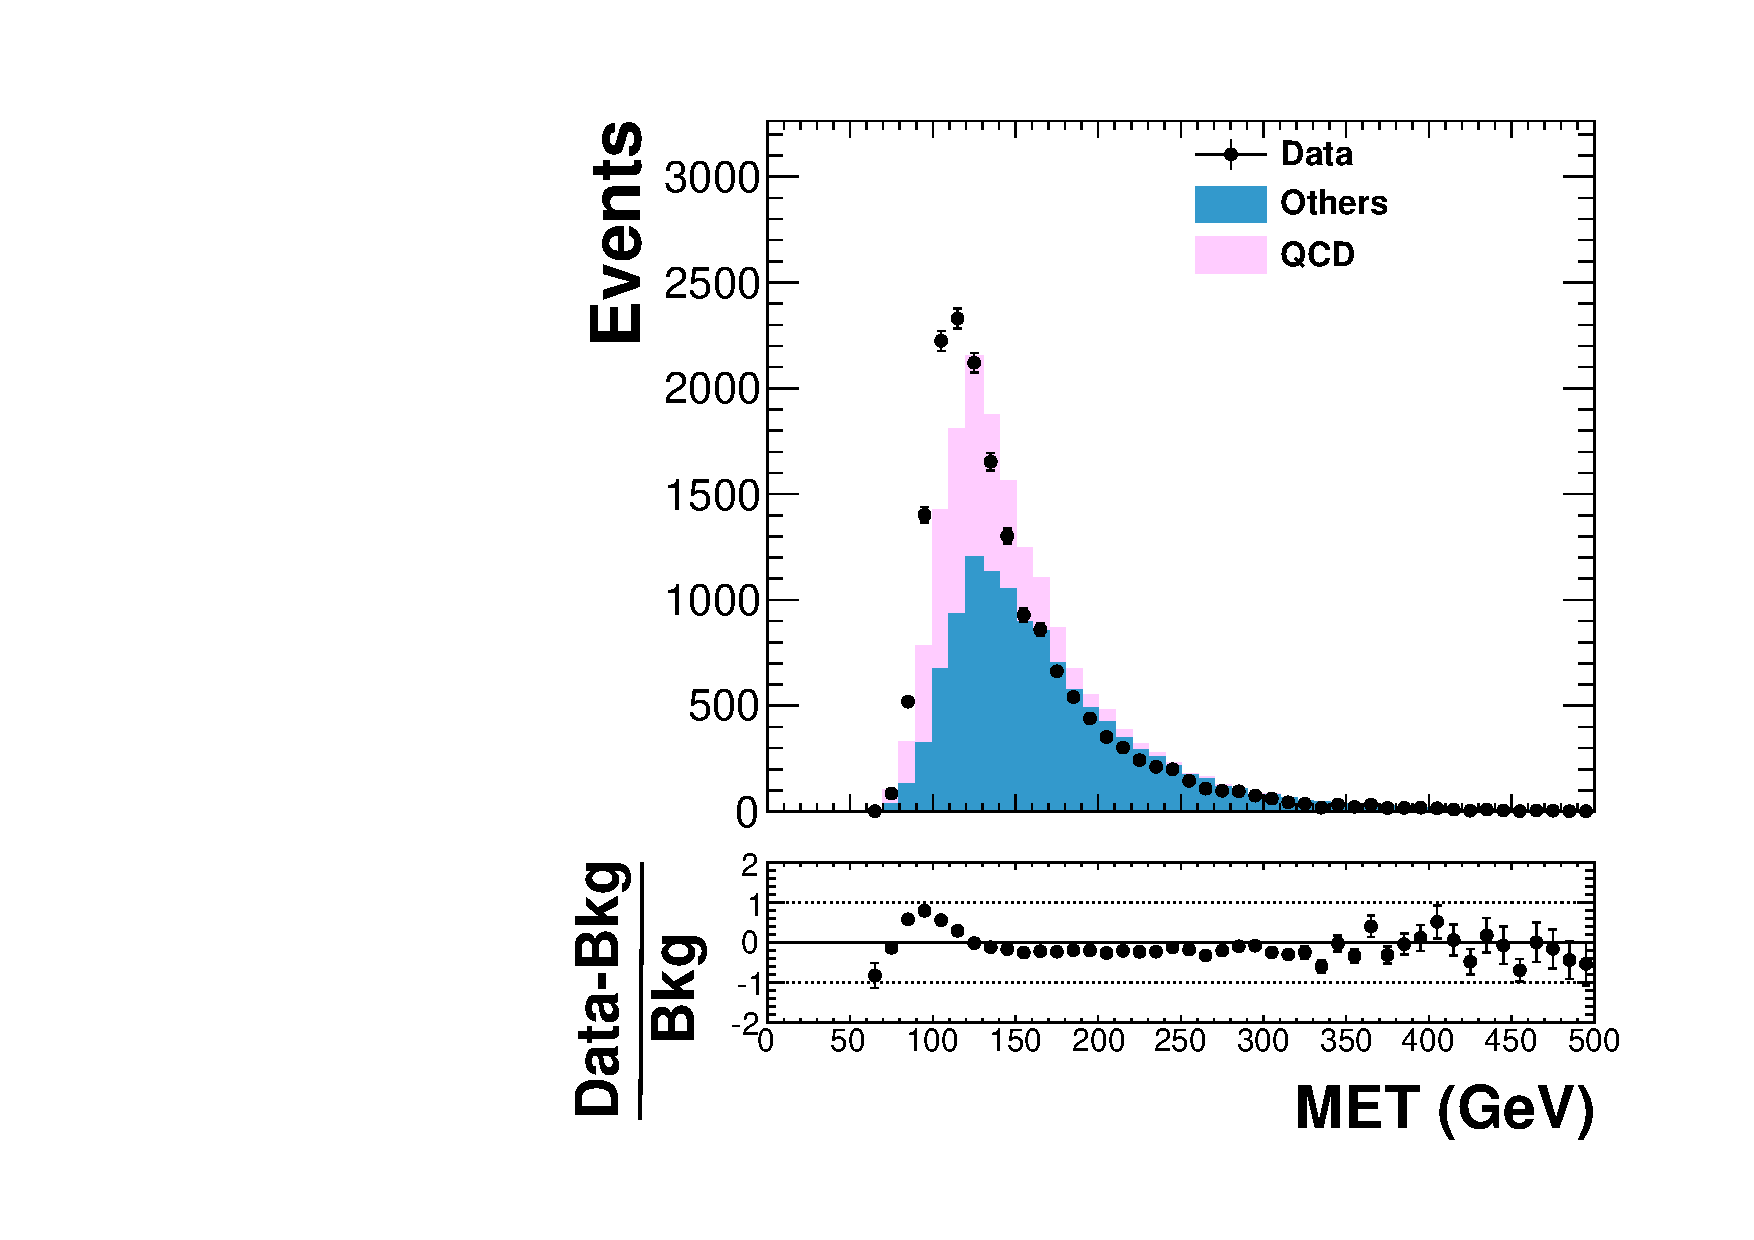
\includegraphics[width=0.45\linewidth]{Chapter06/QCD_VBFMET_Samples/PreSelection/Images//DEta3p6_MetSig3p0_MinDPhiJetsMet1p5/met.pdf}}
\subfloat[]{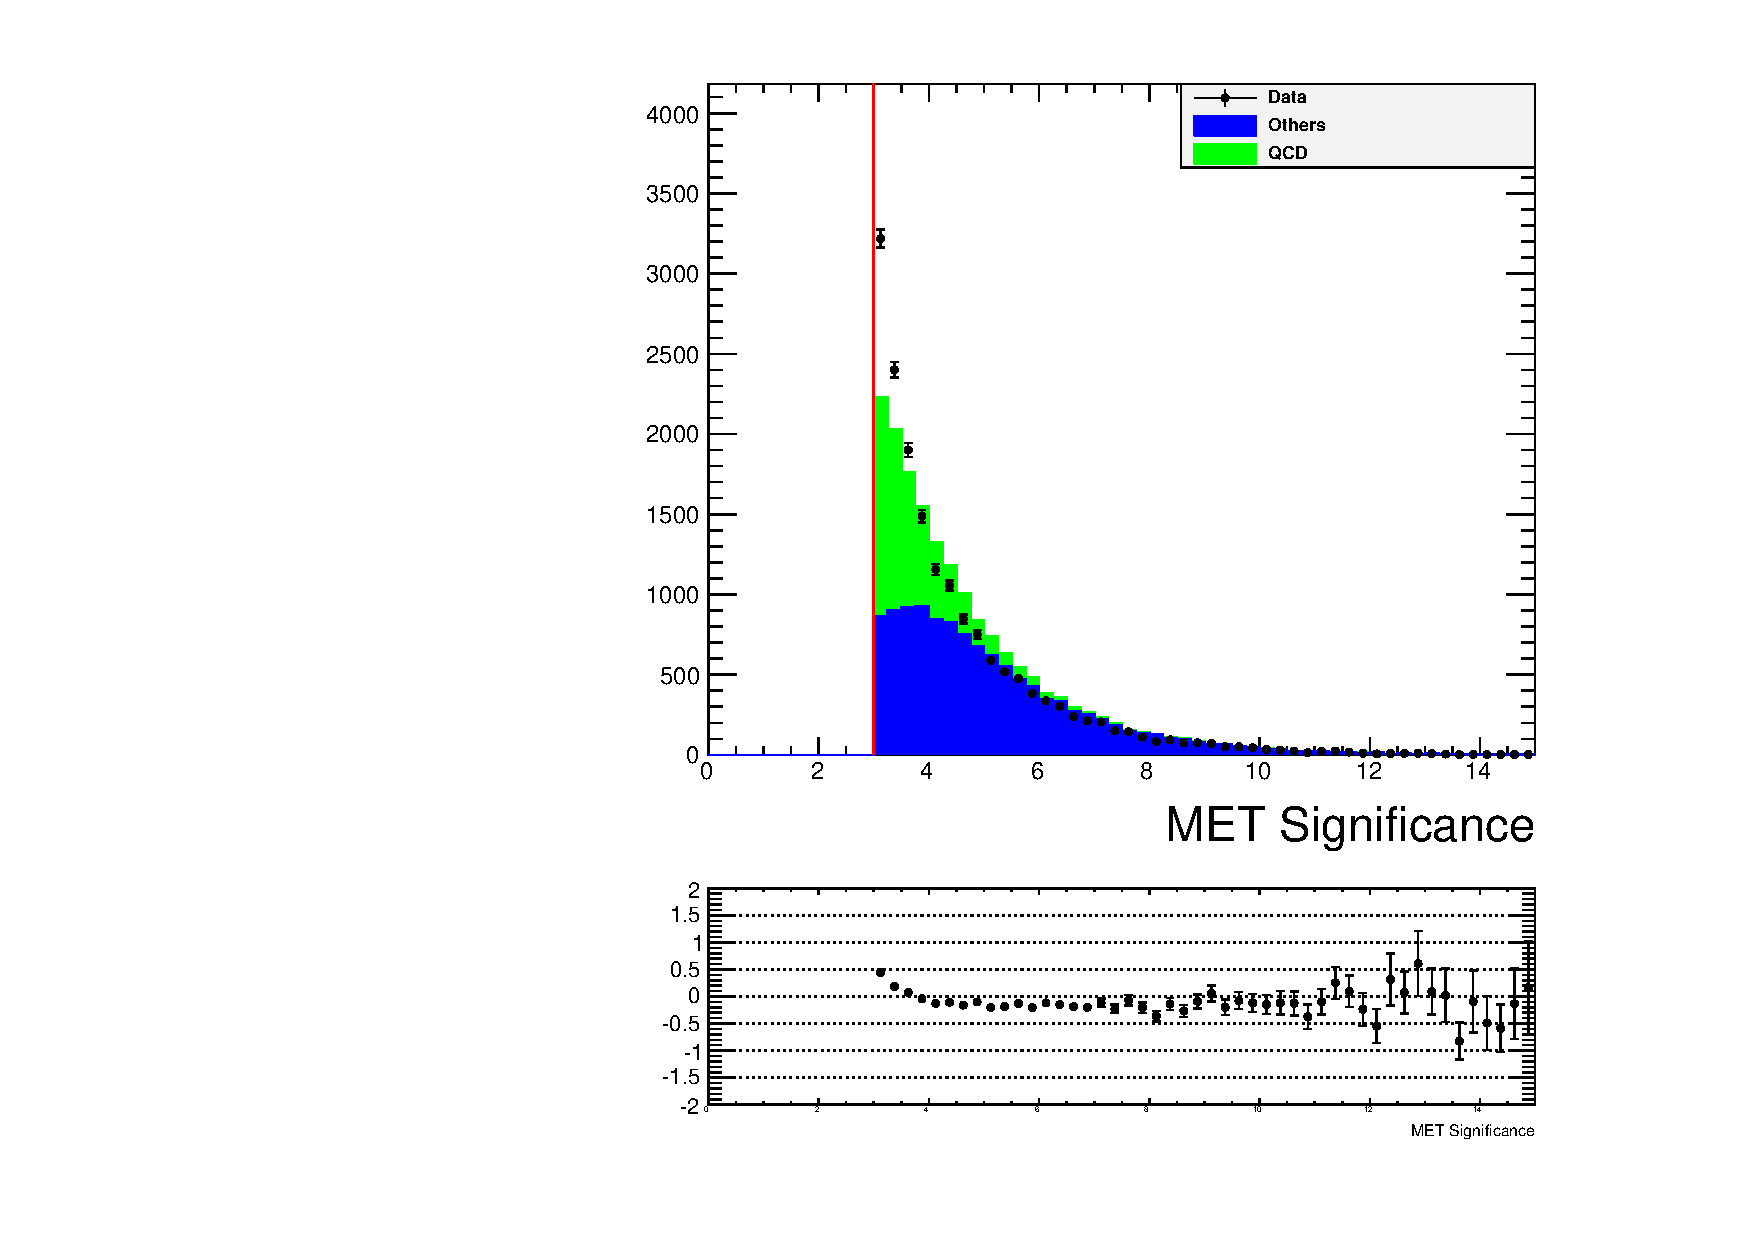
\includegraphics[width=0.45\linewidth]{Chapter06/QCD_VBFMET_Samples/PreSelection/Images//DEta3p6_MetSig3p0_MinDPhiJetsMet1p5/metSig.pdf}} \\
\caption{Plots of the the number of events for some of the key analysis variables after the proposed pre-selection using \gls{MC} simulation including the new \gls{QCD} multi-jet samples and 19.8 $fb^{-1}$ of data. Plot are, (a) dijet invariant mass, (b) hadronic energy total, (c) dijet $\Delta\phi$, (d) dijet $\Delta\eta$, (e) \gls{MET} and (f) \gls{MET} significance. Where red vertical lines can be seen they represent the applied cut by the pre-selection.}
\label{FIGURE:PreparationParkedDataAnalysis_QCDVBFMET_PreSectionVariables}
\end{figure}

Data description by the \gls{MC} event samples was seen as acceptable in all variables to proceed with further studies. The biggest observed discrepancies were observed at low values of \gls{MET} and \gls{MET} significance and high values of dijet $\Delta\eta$.

Unfortunately, when analysing the control regions already defined for the \textit{prompt analysis} with the additional pre-selection requirements the agreement became unacceptable for many variables, making it not possible to use this samples for shape comparison of \gls{BDT} training. The new \gls{QCD} multi-jet samples had special difficulty describing events where the \gls{MET} was aligned with a jet axis which points to \gls{MET} miss measurement. Although, this \gls{QCD} multi-jet event samples could not fully describe this component of data they still model a significant part this background and have been used to study new variables to attempt to suppress at least those types of events. 

% To force plots to be in this section
\clearpage

%%%%%%%%%%%%%%%%%%%%%%%%%%%%%%%%%%%%%%%%%%%%%%%%%%%%%%%%%%%%%%%%%%%%%%%%%%%%%%%%%%%%
%%% SECTION
%%%%%%%%%%%%%%%%%%%%%%%%%%%%%%%%%%%%%%%%%%%%%%%%%%%%%%%%%%%%%%%%%%%%%%%%%%%%%%%%%%%%
\section{Dijet-MET system topological variables}
\label{SECTION:PreparationParkedDataAnalysis_DijetMETSystemVars}
% 18 Months report was on the Sep 9 2013
% 
% /home/hep/jca10/work/vbfinv/ws04/CMSSW_5_3_11/src/UserCode/ICHiggsTauTau/Analysis/HiggsNuNu/PLOTS_mjj1200_dijetFrac/nunu/MET130/n_vtx_2012_DijetFraction_log.pdf
% Looks like plots are from Jun 25 2013
% 
% FOUND FILE: This is the file used in the plots for the 18 months report
% /home/hep/jca10/work/vbfinv/ws04/CMSSW_5_3_11/src/UserCode/ICHiggsTauTau/Analysis/HiggsNuNu/output_mjj1100_dijetFrac/nunu/MET130/MC_VBF_HToZZTo4Nu_M-120.root
% 
% /vols/cms02/jca10/work/ws01/CMSSW_5_3_11/src/UserCode/ICHiggsTauTau/Analysis/HiggsNuNu/plots/DPhiSIGNAL_CJVpass/dijetMet/dijetFrac_htMET.png
% Looks like plots are from Feb 20 2014


% 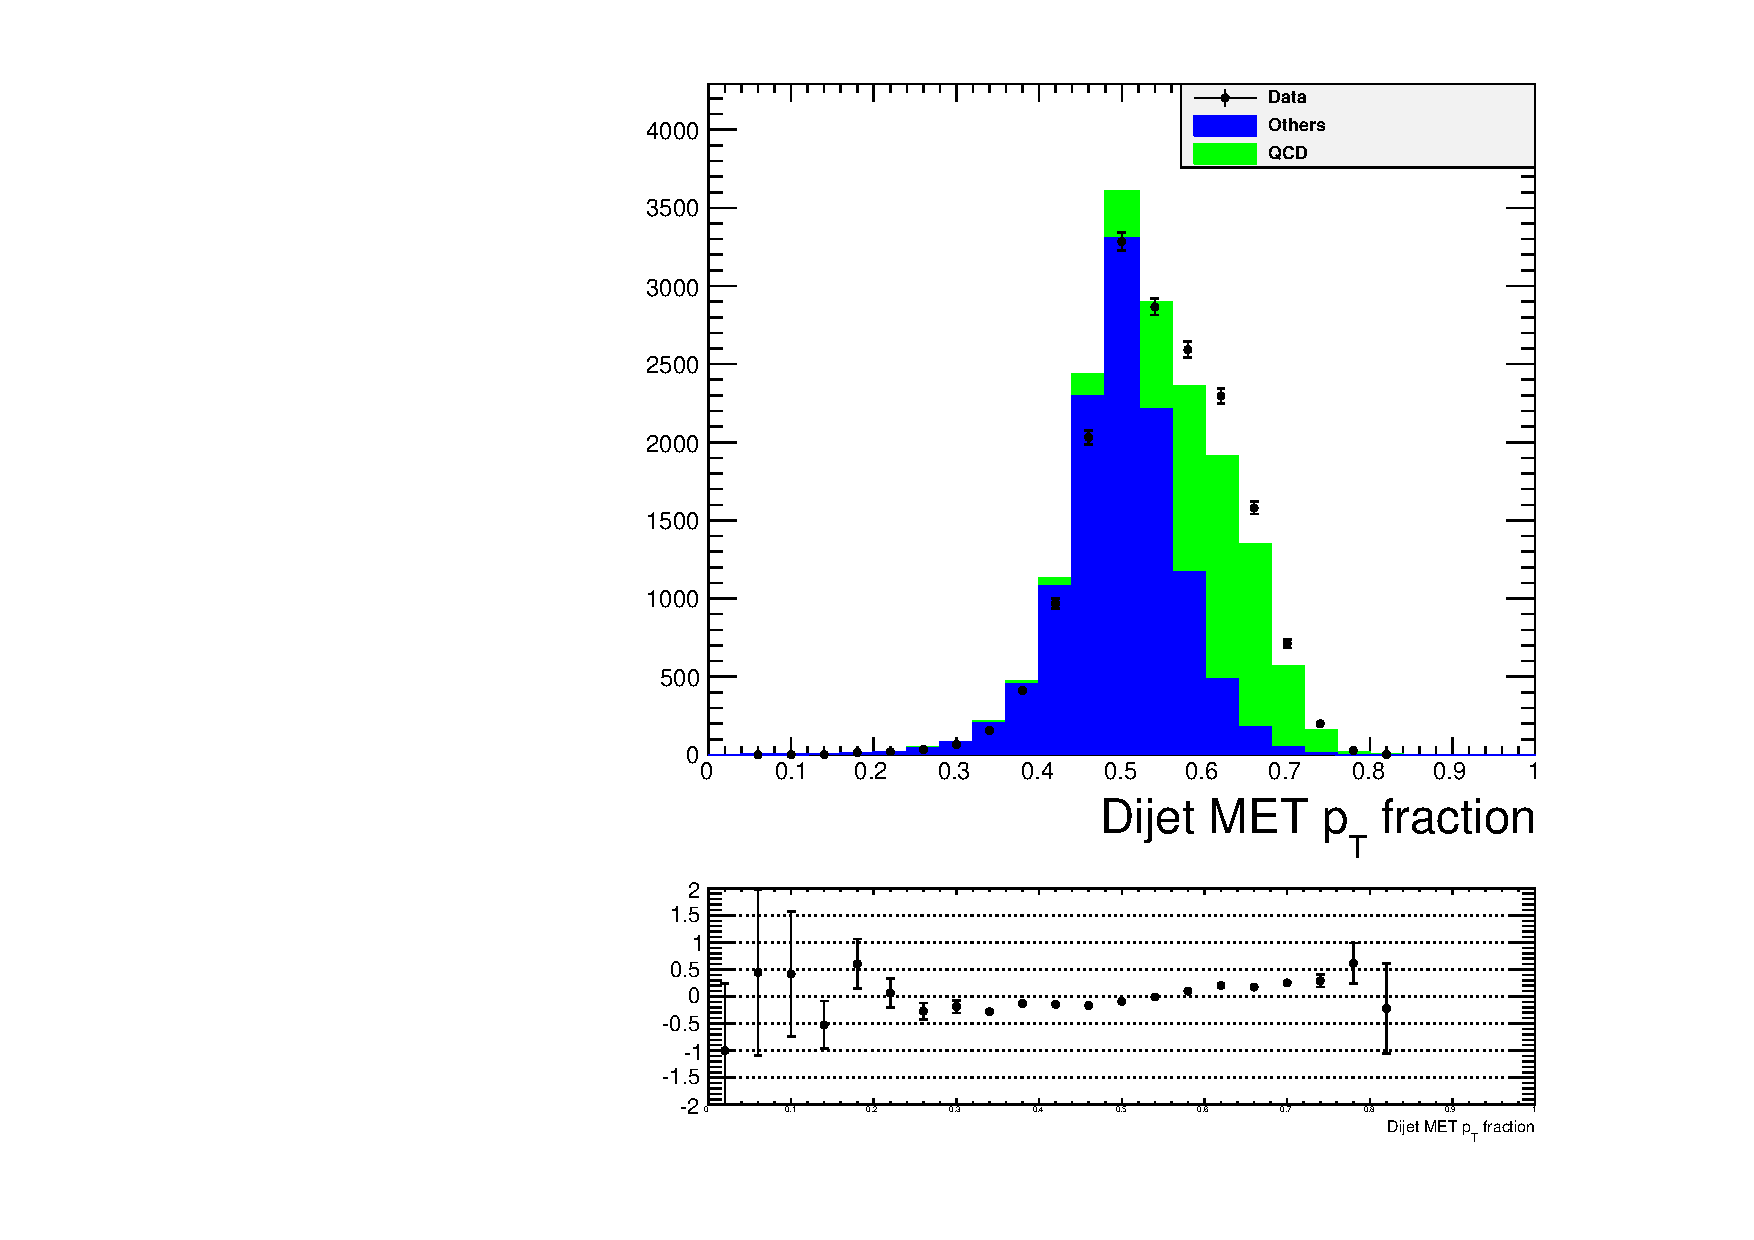
\includegraphics[width=0.48\linewidth]{Chapter06/QCD_VBFMET_Samples/PreSelection/Images//DEta3p6_MetSig3p0_MinDPhiJetsMet1p5/dijetmet_ptfraction.pdf}


%%%%%%%%%%%%%%%%%%%%%%%%%%%%%%%%%%%%%%%%%%%%%%%%%%%%%%%%%%%%%%%%%%%%%%%%%%%%%%%%%%%%
%%% SECTION
%%%%%%%%%%%%%%%%%%%%%%%%%%%%%%%%%%%%%%%%%%%%%%%%%%%%%%%%%%%%%%%%%%%%%%%%%%%%%%%%%%%%
\section{Track distribution variables}
\label{SECTION:PreparationParkedDataAnalysis_TrackDistributionVariables}

% 20140603_ICVBFHiggs_JPela.pdf
% /afs/cern.ch/user/p/pela/work/cms/vbfinv/ws03/CMSSW_5_3_11/src/VBFHiggsToInvisible/VariableAnalyser/python/PowhegSignal_cfi.py
% Plots remade here:
% /afs/cern.ch/user/p/pela/work/cms/vbfinv/ws03/slc6/CMSSW_5_3_11/src/VBFHiggsToInvisible/VariableAnalyser/results/

One of the important features of \gls{VBF} processes is that there is no colour connection between the outgoing quark jets. Since \gls{QCD} multi-jet processes do have colour connection, it is expected that \gls{QCD} background events will have hadronic activity between the leading jets. Motivating the use of a central jet veto in the Run I prompt analysis. Events were vetoed if a jet identified as coming from \gls{PV} with enough \pt was found between the two leading jets. But colour connection can result simply in a spread of energy in the event which may be clustered into \gls{PU} jets or remain unclustered. Also by having a minimum \pt requirement on a single veto jet may result in accepting events where multiple jets coming from the \gls{PV} are present with low \pt, but if combined would pass the veto threshold.

For colour connected jets it is expected that a significant amount tracks coming from the primary vertex would be spread in the event specially between the selected jets. It forward physics analysis with similar unconnected dijet signal topologies it is common to use variables like the fraction of tracks inside the selected jets to isolate the signal from background \cite{ARTICLE:AnalysisDiffractiveJets}. Considering tracks has the advantages of not depending on jet clustering or veto jet selection and using directly the excellent resolution of the \gls{CMS} inner tracking system. 

Two variables were considered for inclusion in a cut or \gls{MVA} based signal selection criteria, the fraction of track coming from the \gls{PV} contained inside the selected jets and the fraction of summed momentum associated with tracks from the \gls{PV} contained inside the selected jets, $\phi$.

%TODO: Continue here

\begin{figure}[!htb]
\centering
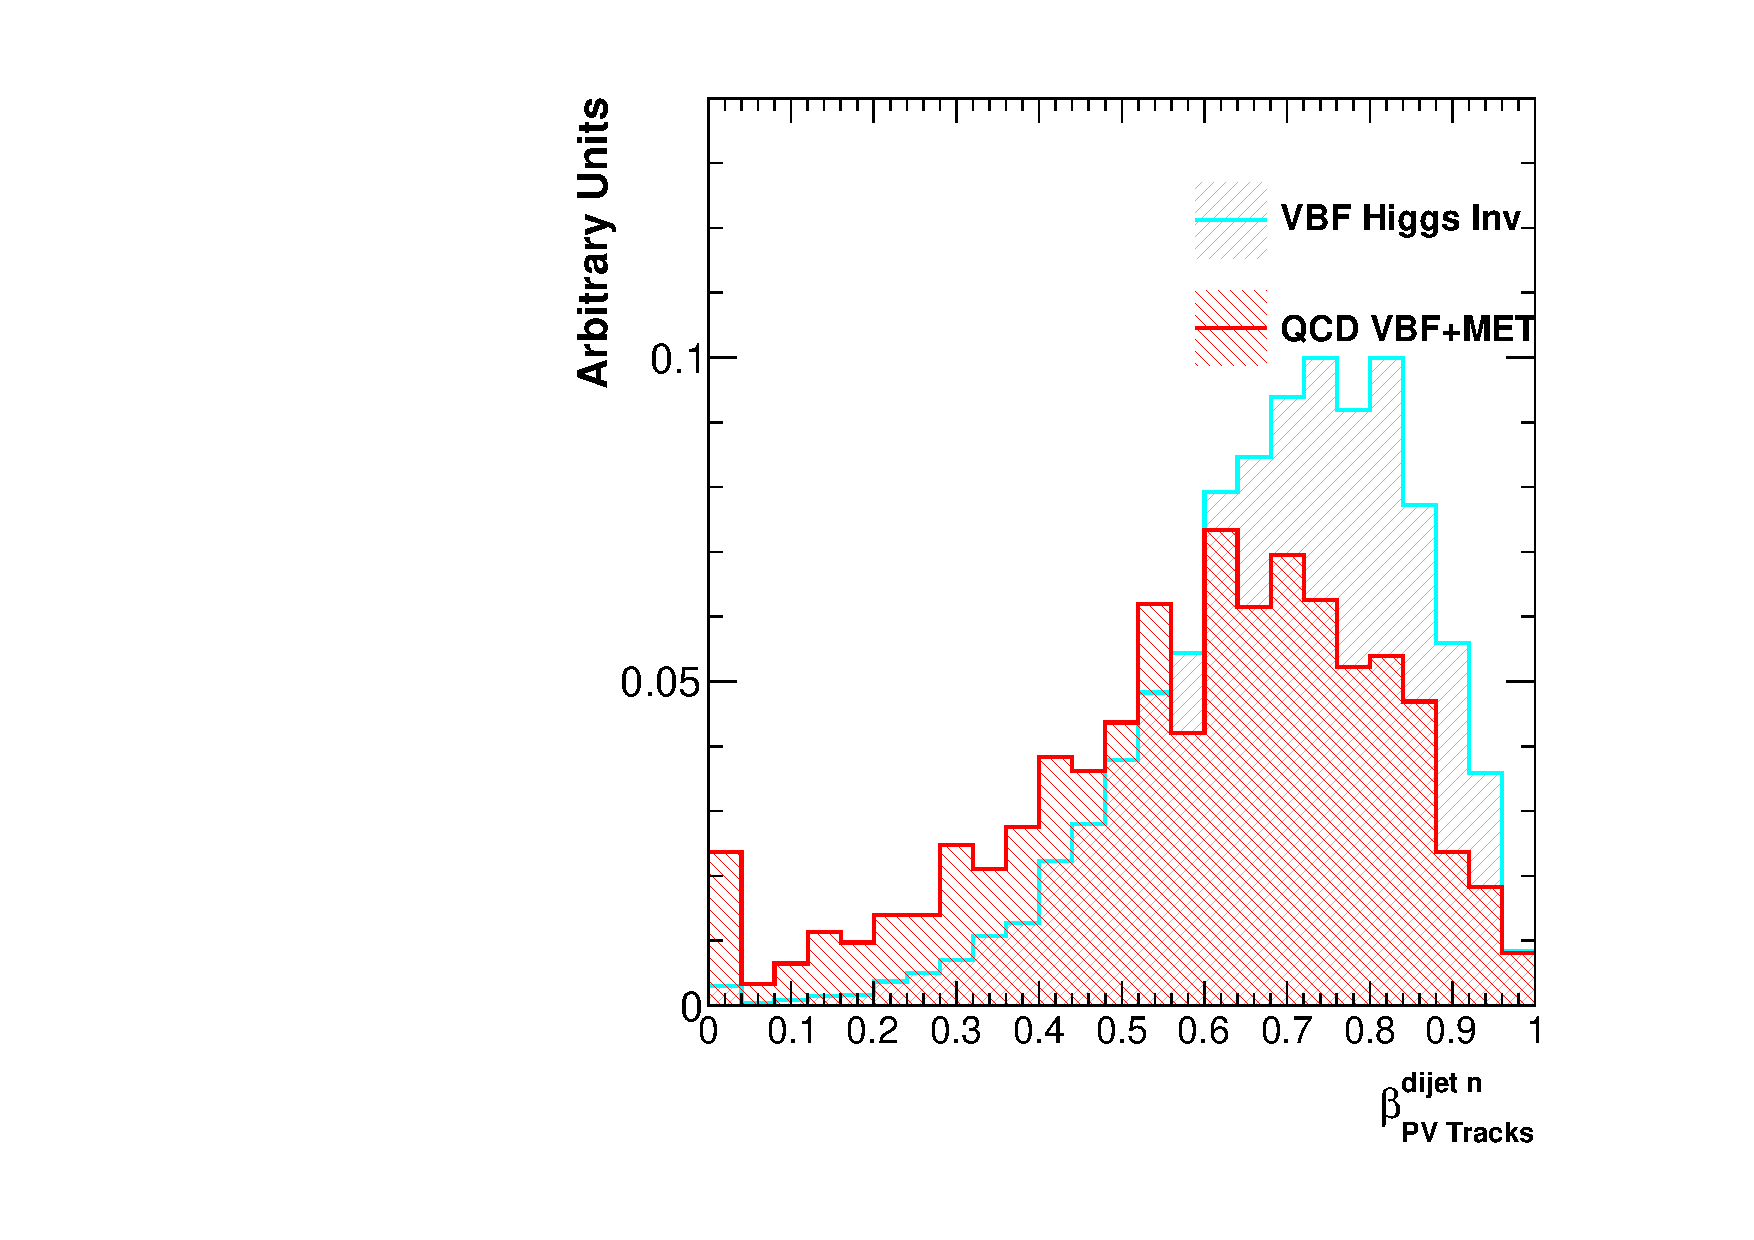
\includegraphics[width=0.45\textwidth]{Chapter06/TrackVariables/Images/Tracks1_TracksNRatio.pdf} 
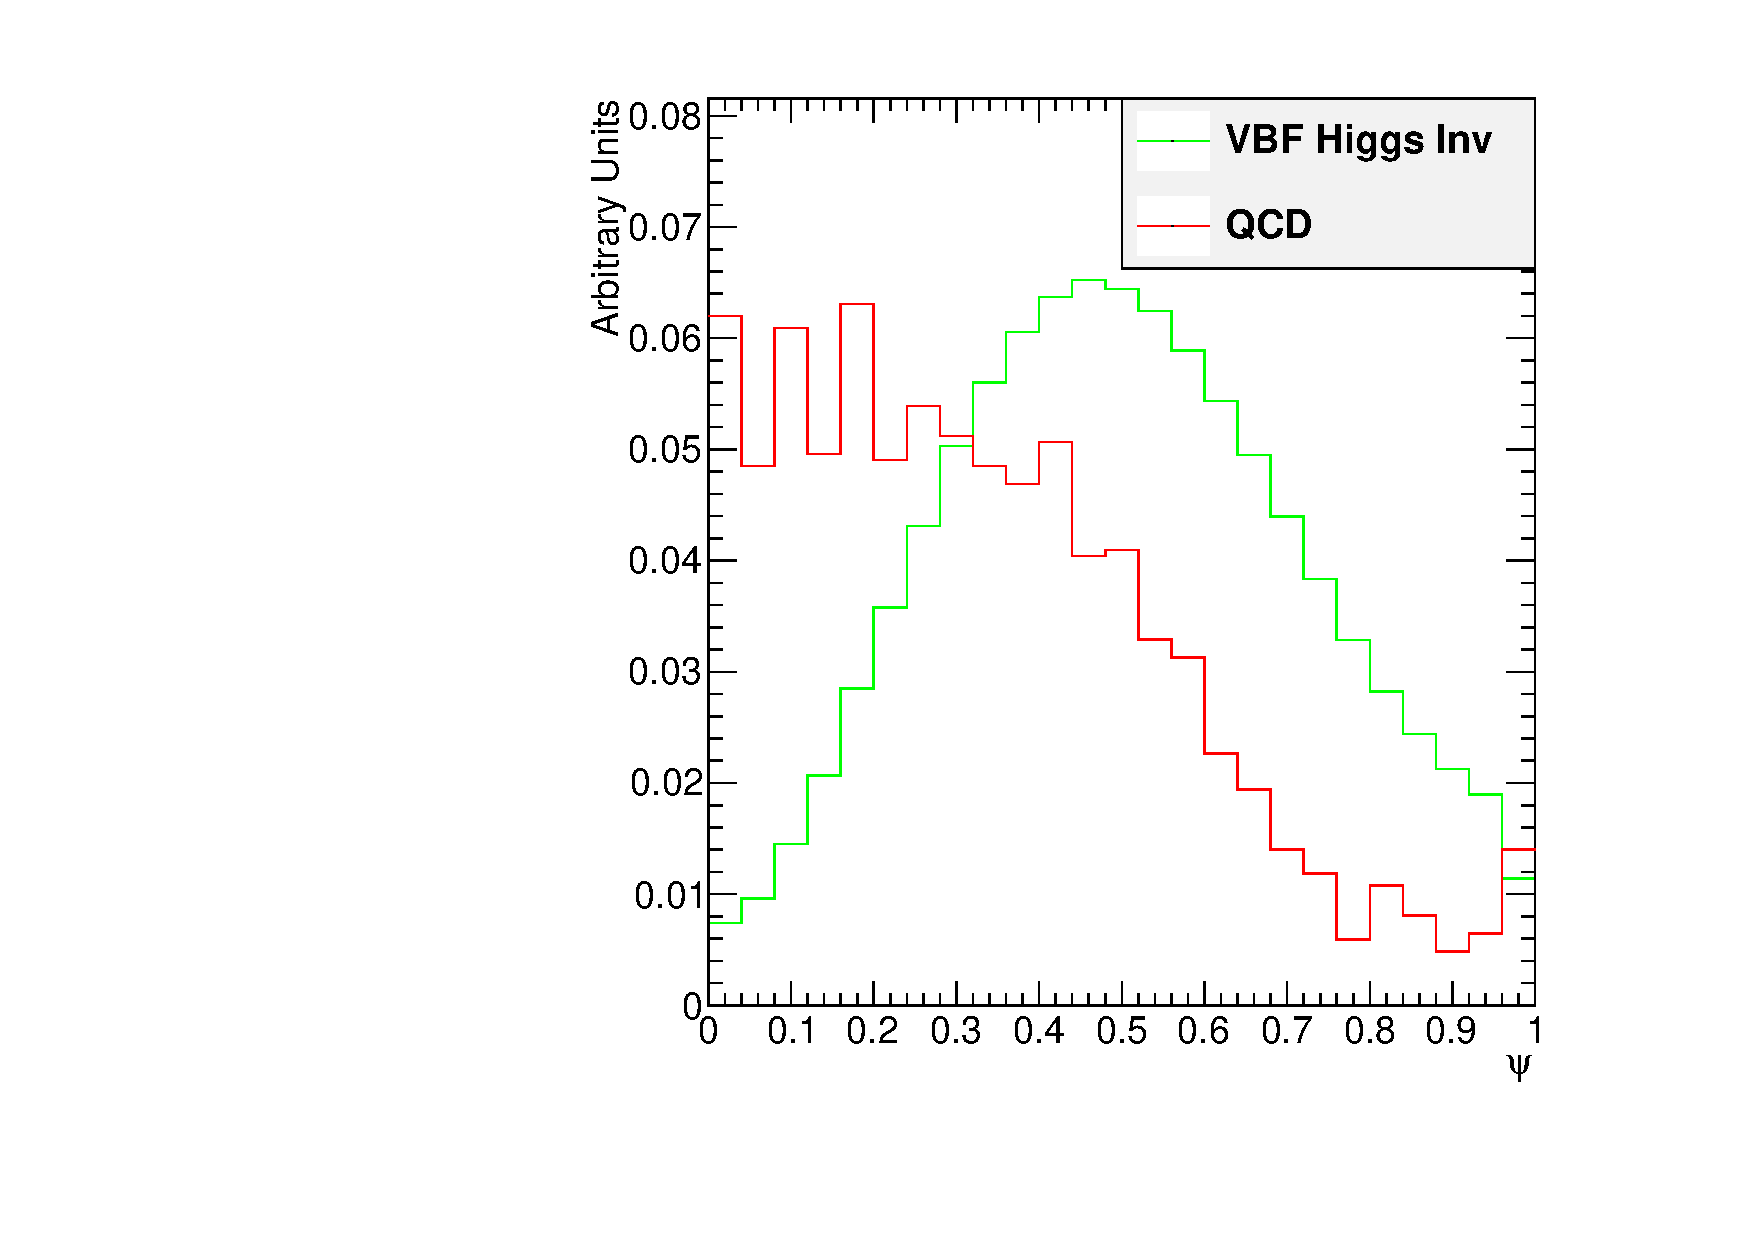
\includegraphics[width=0.45\textwidth]{Chapter06/TrackVariables/Images/Tracks1_TracksERatio.pdf} \\
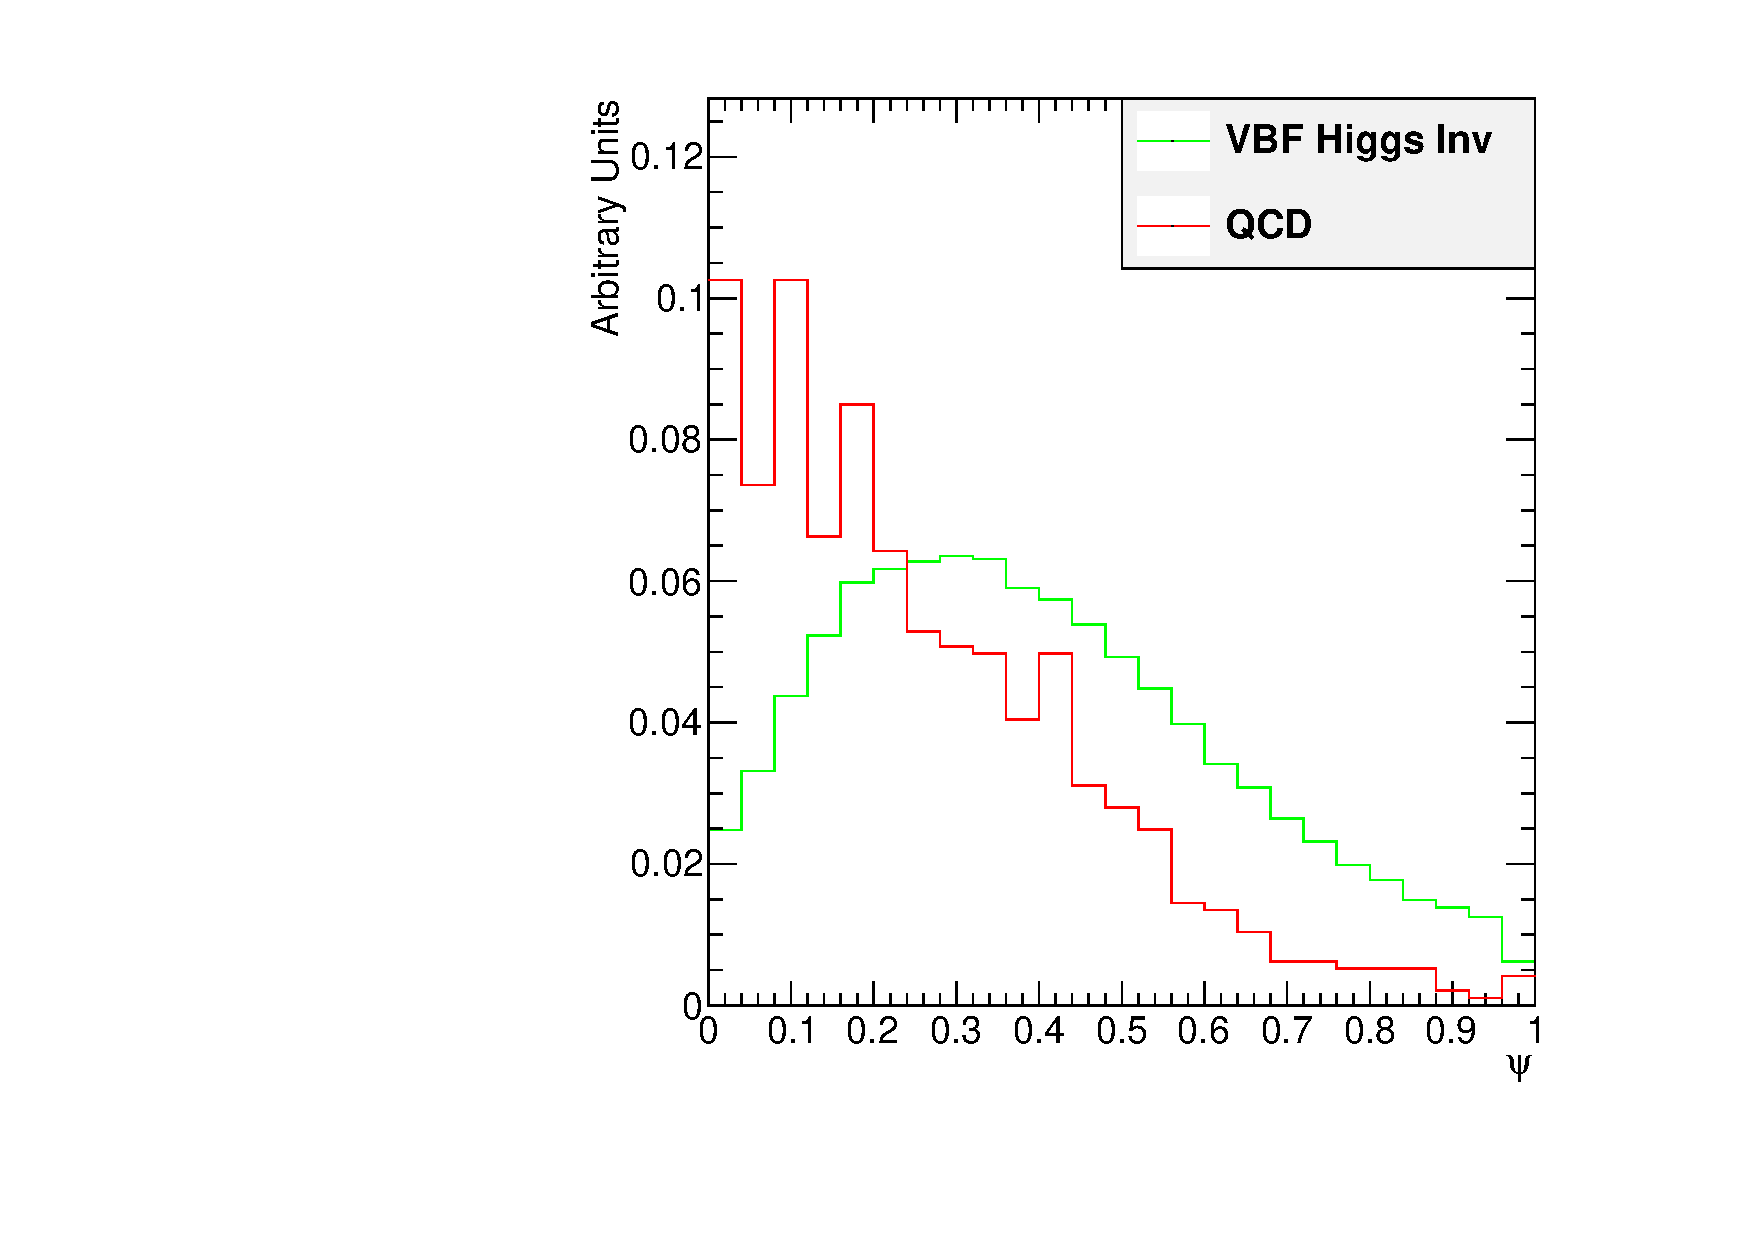
\includegraphics[width=0.45\textwidth]{Chapter06/TrackVariables/Images/Tracks1_CJVPass_TracksERation.pdf}
\caption{TODO}
\label{FIGURE:PreparationParkedDataAnalysis_TrackDistributionVariables_Selection}
\end{figure}

\begin{figure}[!htb]
\centering
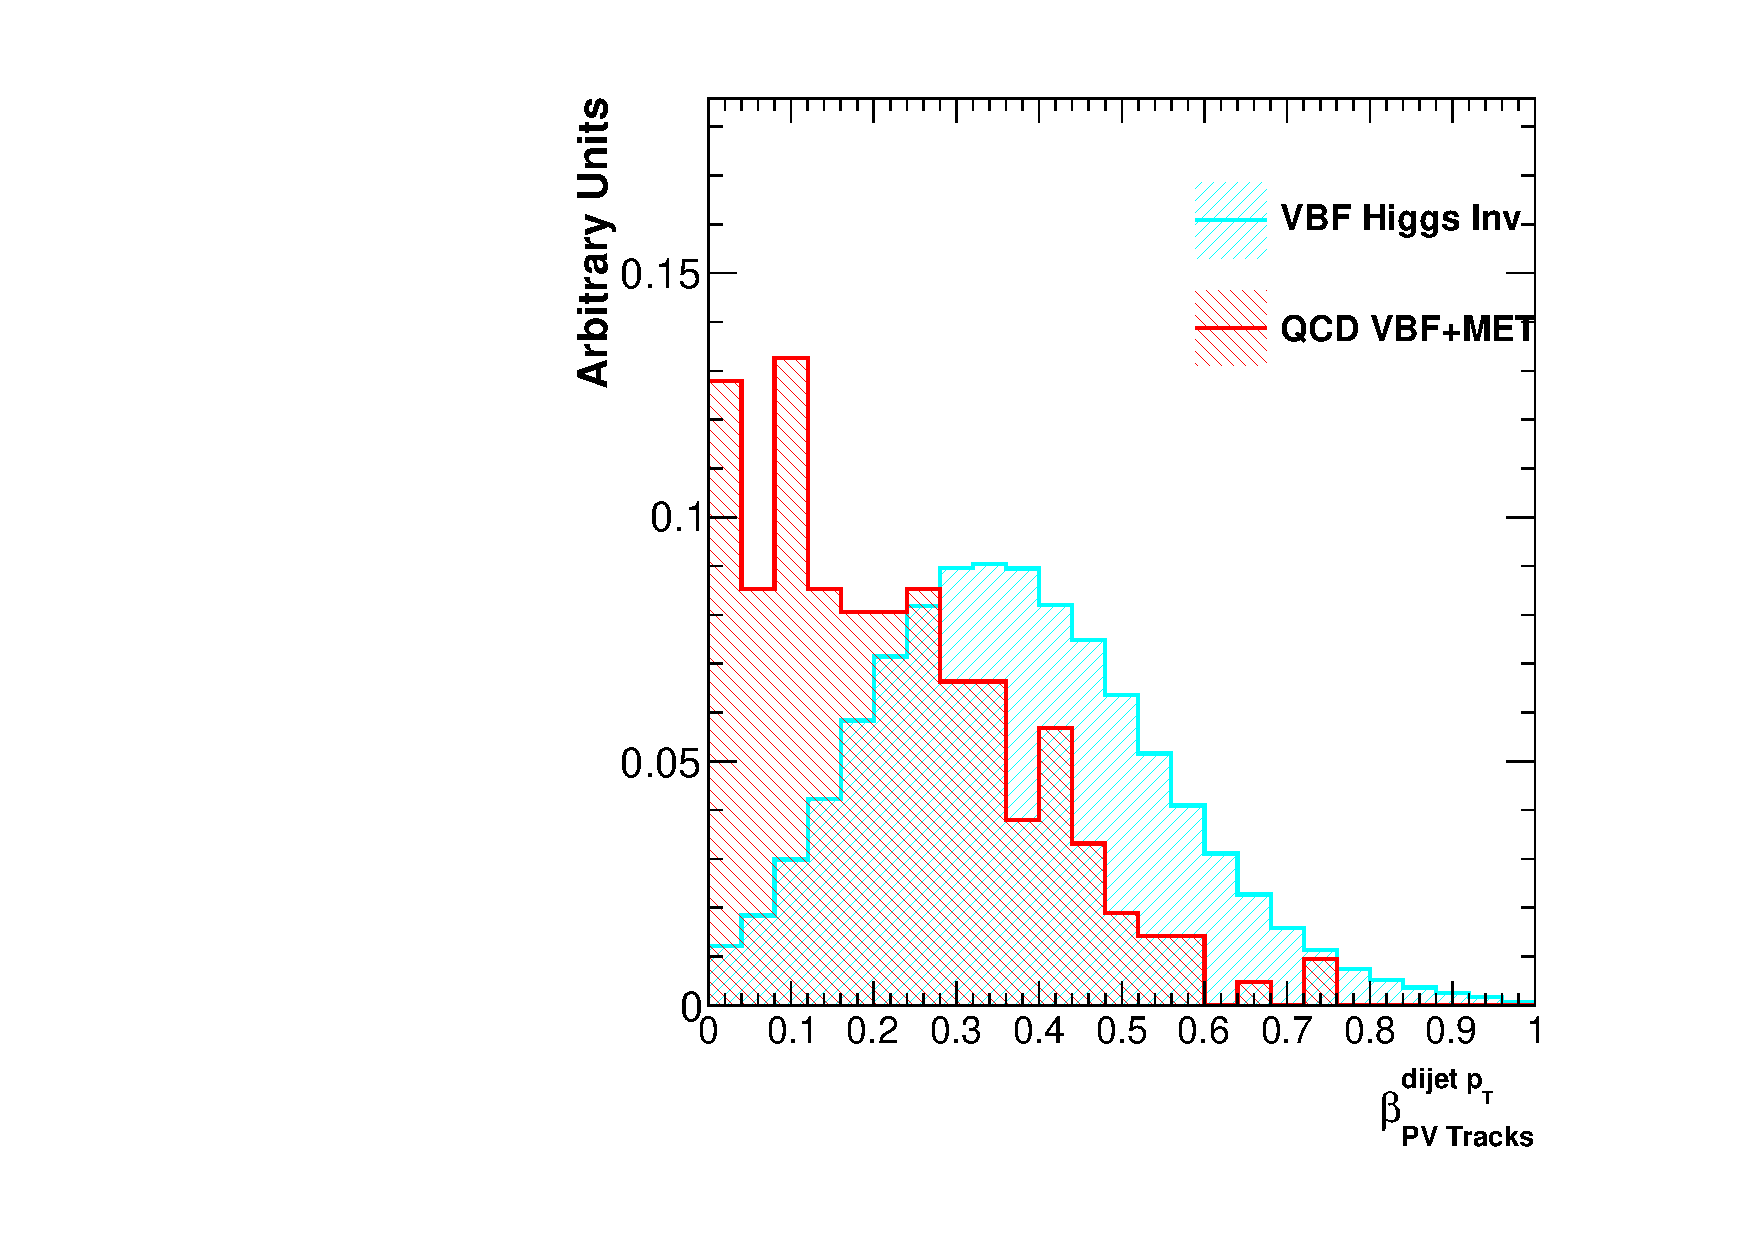
\includegraphics[width=0.45\textwidth]{Chapter06/TrackVariables/Images/BB_Tracks1_TracksERatio.pdf}
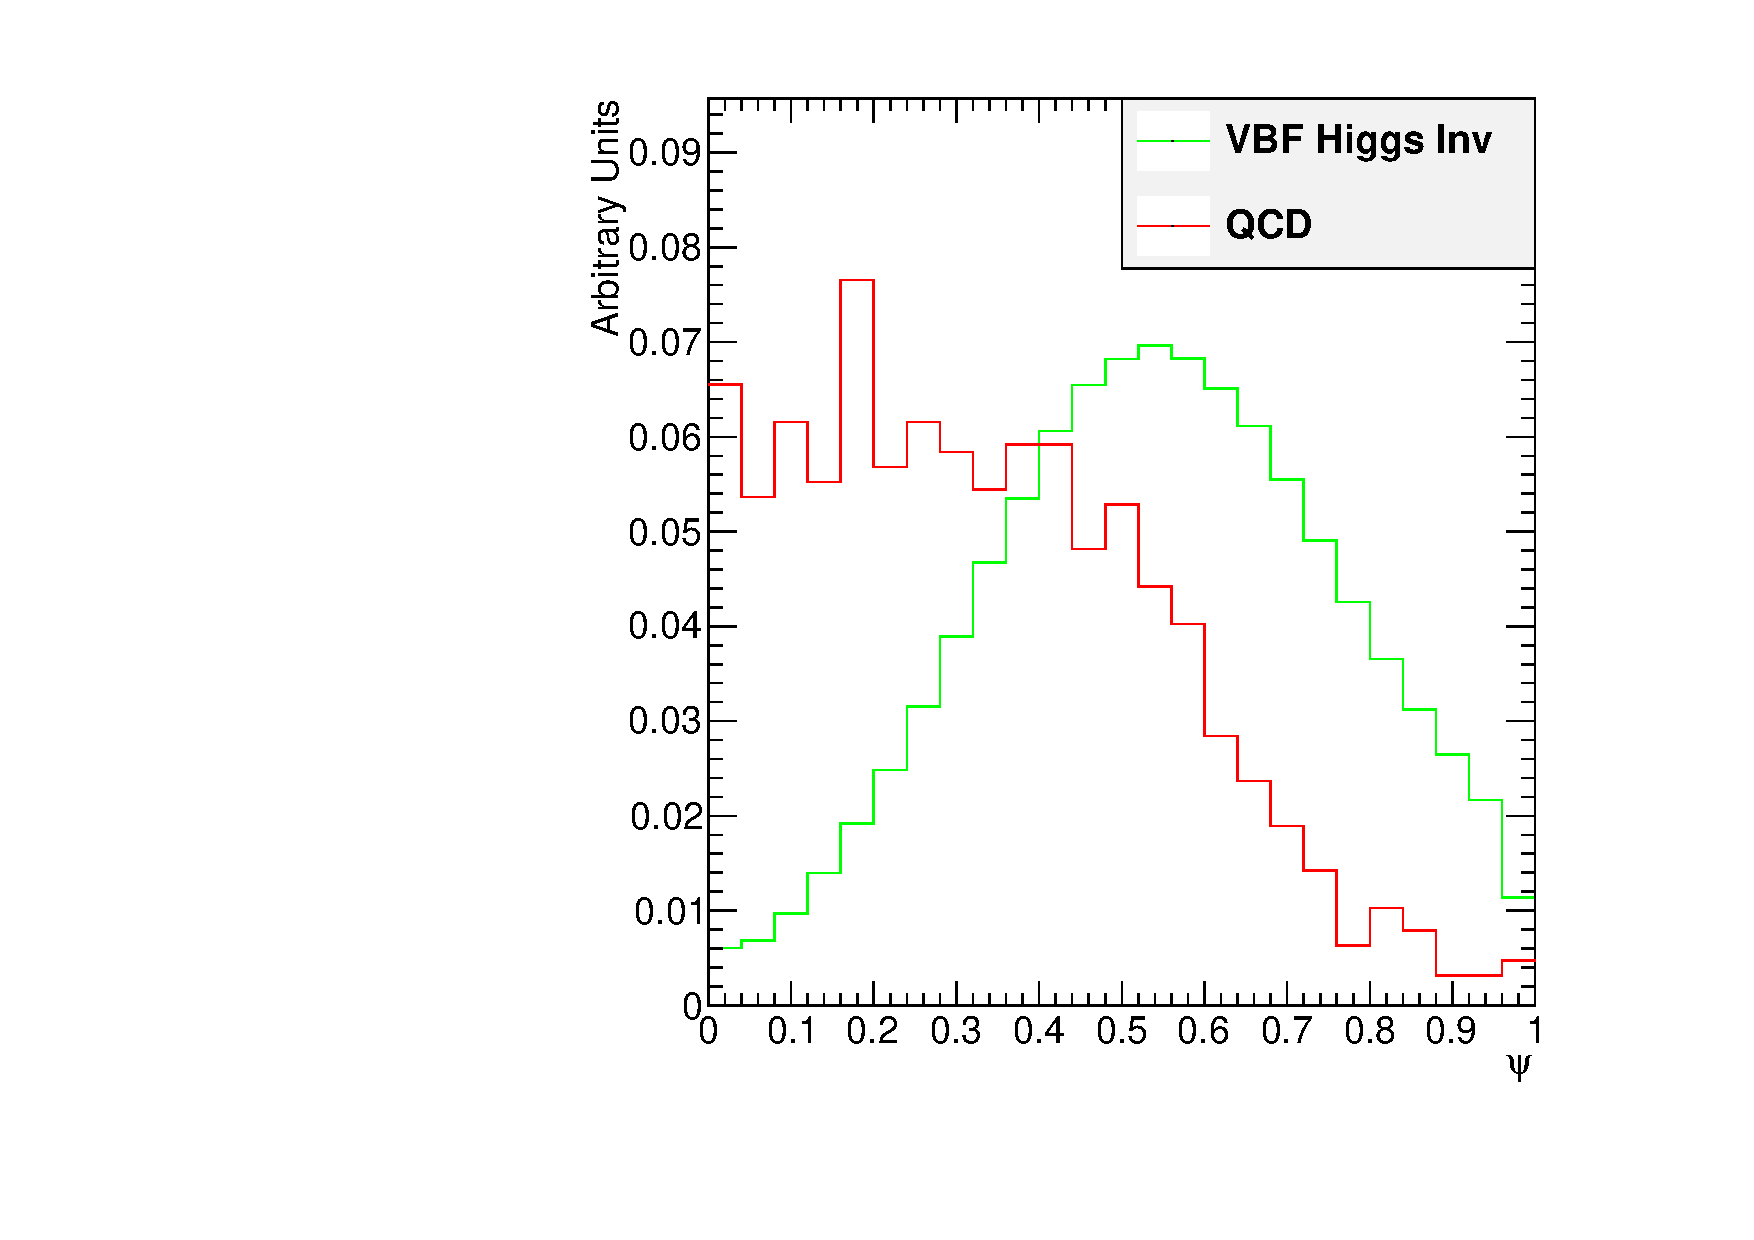
\includegraphics[width=0.45\textwidth]{Chapter06/TrackVariables/Images/BE_Tracks1_TracksERatio.pdf} \\
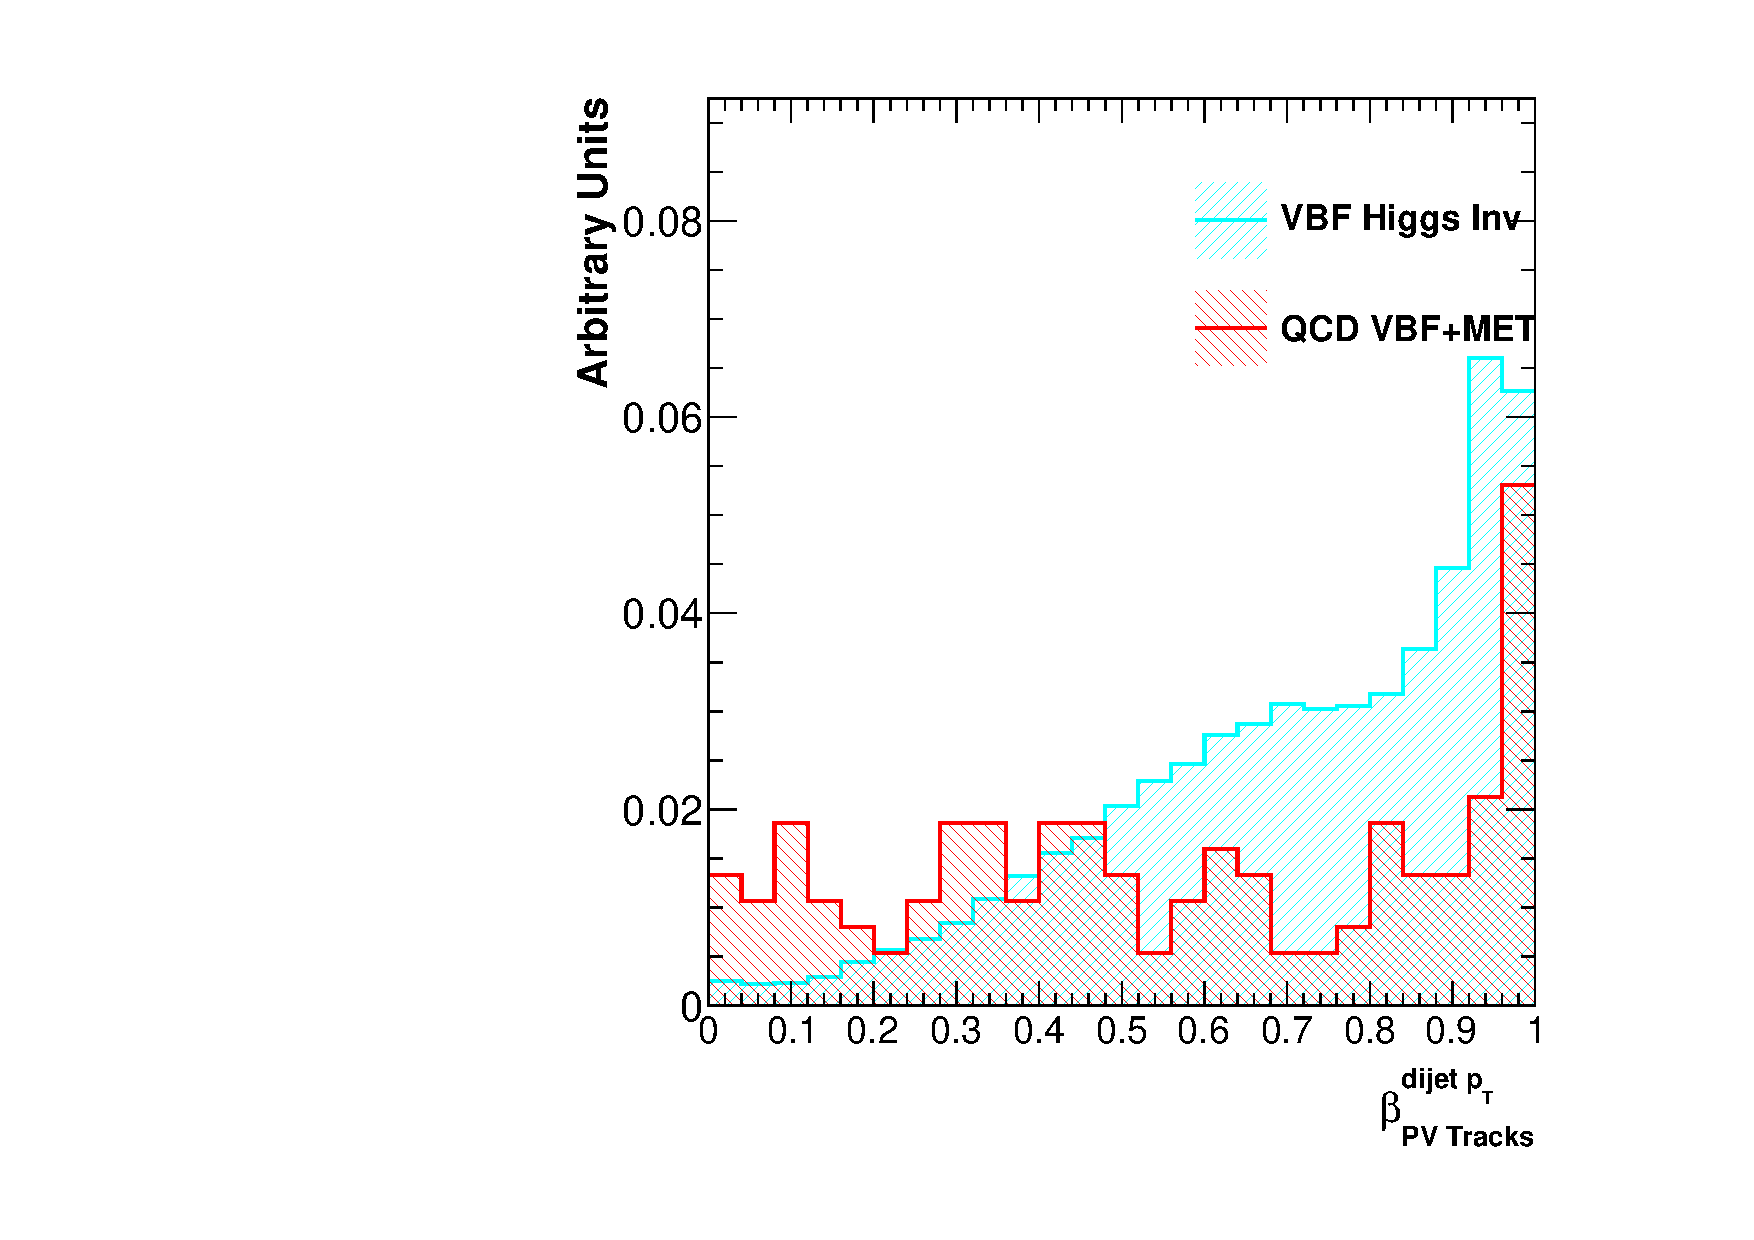
\includegraphics[width=0.45\textwidth]{Chapter06/TrackVariables/Images/EE_Tracks1_TracksERatio.pdf}
\caption{TODO}
\label{FIGURE:PreparationParkedDataAnalysis_TrackDistributionVariables_Acceptance}
\end{figure}

